\documentclass[aspectratio=169]{beamer}
\usetheme{Luebeck}
\setbeamertemplate{headline}{}
\setbeamertemplate{headline}{
  \leavevmode%
  \hbox{%
    \begin{beamercolorbox}[wd=\paperwidth,ht=2.5ex,dp=1.125ex,center]{section in head/foot}%
      \usebeamerfont{section in head/foot}\insertsectionhead
    \end{beamercolorbox}%
  }
}

\usepackage{xcolor}
% Theme colors
\definecolor{myaccent}{RGB}{34,139,34}
\definecolor{mydark}{RGB}{47,79,79}
\definecolor{mywhite}{RGB}{255,255,255}
\definecolor{myblack}{RGB}{30, 30, 30}
\definecolor{darkforest}{RGB}{0,70,30}

\setbeamercolor{structure}{fg=myaccent}
\setbeamercolor{frametitle}{fg=white, bg=darkforest}
\setbeamercolor{title}{fg=mywhite}
\setbeamercolor{subtitle}{fg=mywhite}
\setbeamercolor{author}{fg=myblack}
\setbeamercolor{date}{fg=myblack}

\usepackage[sfdefault]{FiraSans}
\usepackage{inconsolata}

\setbeamertemplate{footline}{
  \leavevmode%
  \hbox{\begin{beamercolorbox}[wd=.5\paperwidth,ht=2.5ex,dp=1.125ex,leftskip=.3cm plus1fill,rightskip=.3cm]{author in head/foot}%
    \usebeamerfont{author in head/foot}\insertshortauthor~(\insertshortinstitute)
  \end{beamercolorbox}%
  \begin{beamercolorbox}[wd=.5\paperwidth,ht=2.5ex,dp=1.125ex,leftskip=.3cm,rightskip=.3cm plus1fil]{title in head/foot}%
    \usebeamerfont{title in head/foot}\insertshorttitle\hfill\insertframenumber\,/\,\inserttotalframenumber
  \end{beamercolorbox}}%
  \vskip0pt%
}

\usepackage[spanish]{babel}
\usepackage[T1]{fontenc}
\usepackage{svg}
\usepackage{tikz}
\usepackage{etoolbox}
\usepackage{graphicx}
\usetikzlibrary{tikzmark, calc}
\usepackage{multicol}

\newcommand{\watermark}{
  \begin{tikzpicture}[remember picture,overlay]
    \node[anchor=south east,opacity=0.1,xshift=-1pt,yshift=12pt] at (current page.south east) {
      \includesvg[width=1.5cm]{UN_emblem_blue.svg}
    };
  \end{tikzpicture}
}

% Other colors
\definecolor{skyblue}{HTML}{87CEEB}
\definecolor{tomato}{HTML}{FF6347}
\definecolor{gold}{HTML}{FFD700}
\definecolor{peachorange}{HTML}{FC8D59}
\definecolor{indianred2}{HTML}{EE6363}
\definecolor{darkslategray3}{HTML}{79CDCD}

\title{Barrios populares en Argentina}

\subtitle{Sobre la calidad de vida y diferencias en la condición de tenencia}

\author{Ariel Leonardo Fideleff}

\institute[AA - Business Intelligence (Conosur)]{Advanced Analytics - Business Intelligence (Conosur)\\\vspace{4pt}\textbf{Dirigido al Consejo Económico y Social}\vspace{-12pt}}

\date{}

\titlegraphic{\includesvg[width=1.5cm]{UN_emblem_blue.svg}}

\beamertemplatenavigationsymbolsempty

\begin{document}
    \frame{\titlepage}

    \setbeamertemplate{background}{\watermark}

    \begin{frame}
        \tableofcontents
    \end{frame}

    \section{Sobre los datos}
    \begin{frame}
        \tableofcontents[currentsection]
    \end{frame}

    \begin{frame}{Relevamiento de Condiciones Habitacionales 2022}
        \begin{minipage}{.64\linewidth}
            \setlength{\leftmargini}{8pt}
            \begin{itemize}
                \item<2-> Datos recopilados por \textbf{La Poderosa} en 2022
                \item<3-> Encuestas de 23 barrios populares de la República Argentina
                \item<4-> 7 principales regiones económicas del país
                \item<5-> 1222 viviendas totales
            \end{itemize}
        \end{minipage}
        \hfill
        \begin{minipage}{.35\linewidth}
            \only<1,2>{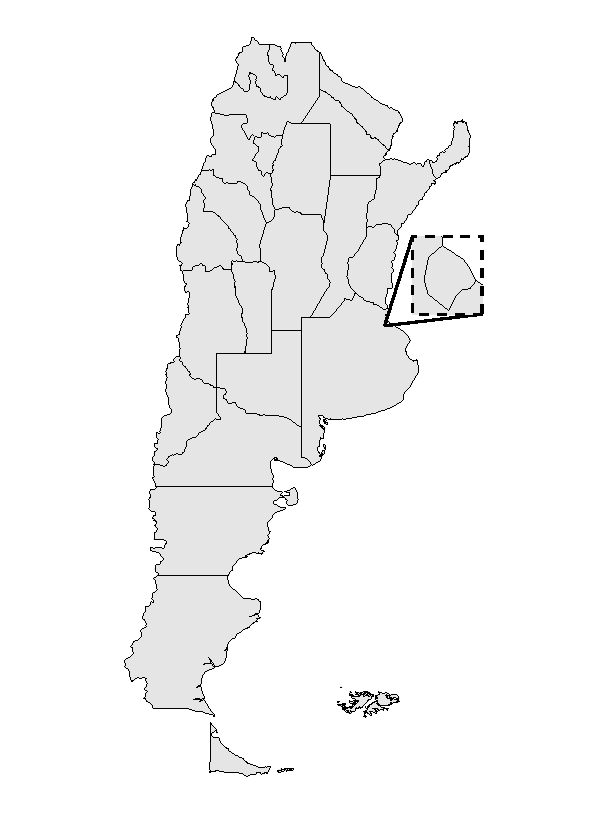
\includegraphics[width=\linewidth]{graficas-pdf/mapa-datos-vacio.pdf}}
            \only<3>{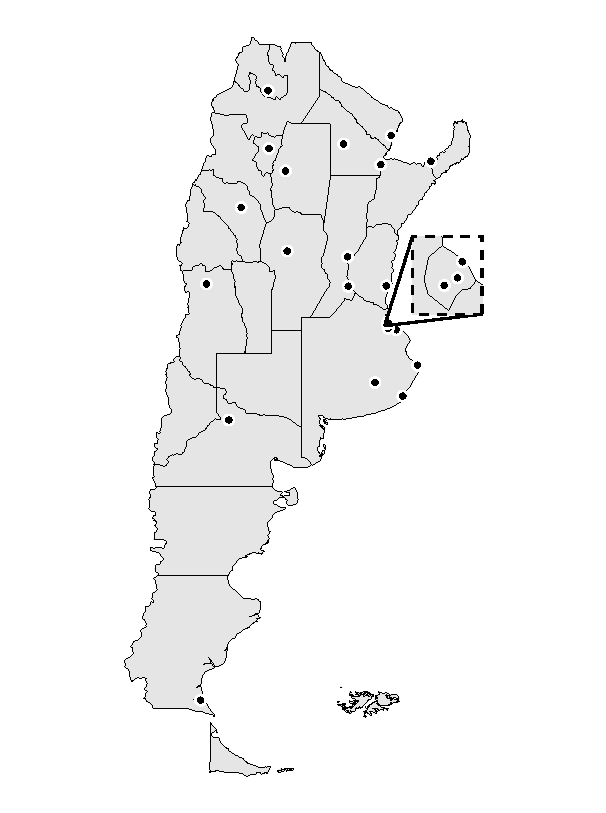
\includegraphics[width=\linewidth]{graficas-pdf/mapa-datos-solo-barrios.pdf}}
            \only<4->{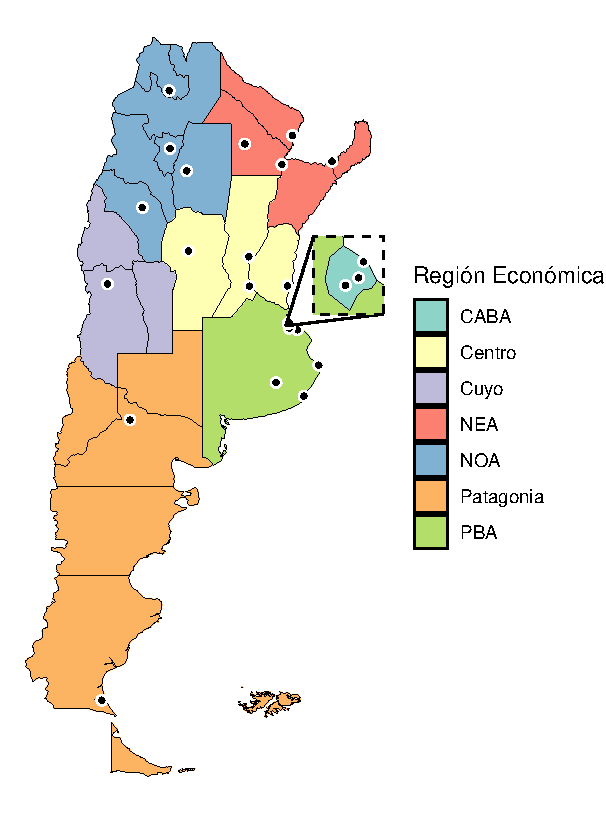
\includegraphics[width=\linewidth]{graficas-pdf/mapa-datos.pdf}}
        \end{minipage}
    \end{frame}

    \section{Motivación del estudio}
    \begin{frame}
        \tableofcontents[currentsection]
    \end{frame}

    \begin{frame}{Los barrios populares por definición}
        \setlength{\leftmargini}{8pt}
        \begin{itemize}
            \item<2-> ¿Cómo se define \textbf{barrio popular}? \uncover<3->{(según ley argentina)}
                \begin{itemize}
                    \item<3-> Viven 8 o más familias agrupadas o contiguas
                    \item<4-> \textit{Más de la mitad de la población no cuenta con \textbf{título de propiedad}, ni acceso regular a 2 o más de los \textbf{servicios básicos}}
                \end{itemize}
            \item<5-> Caso de estudio: \textit{los hogares inquilinos}, y un informe del Ministerio de Desarrollo Social (2021)
                \begin{itemize}
                    \item<6-> \textit{Demografía de la población afectada}:
                        \begin{itemize}
                            \item<7-> ¿\textbf{Antigüedad de residencia}?
                            \item<8-> ¿\textbf{Cantidad de menores} por hogar?
                        \end{itemize}
                \end{itemize}
        \end{itemize}
    \end{frame}

    \begin{frame}{Objetivos}
        Respecto a los barrios relevados:
        \begin{itemize}
            \item<2-> Analizar la calidad de vida y de acceso a los servicios básicos en las viviendas
            \item<3-> Edad del jefe/a del hogar: ¿qué nos dice sobre las familias que habitan?
            \item<4-> Determinar la influencia de la condición de tenencia sobre otras variables
        \end{itemize}
    \end{frame}
    
    \section{Calidad de vida y de acceso a los servicios básicos}
    \begin{frame}
        \tableofcontents[currentsection]
    \end{frame} % TODO: Acortar capaz para respetar tiempo y que sea más "Freytag"? Así al principio es corto y el desarrollo es lo más importante

    \begin{frame}{Hacinamiento}
        \begin{minipage}{.65\linewidth}
            \begin{overlayarea}{\linewidth}{.75\textheight}
                \only<1>{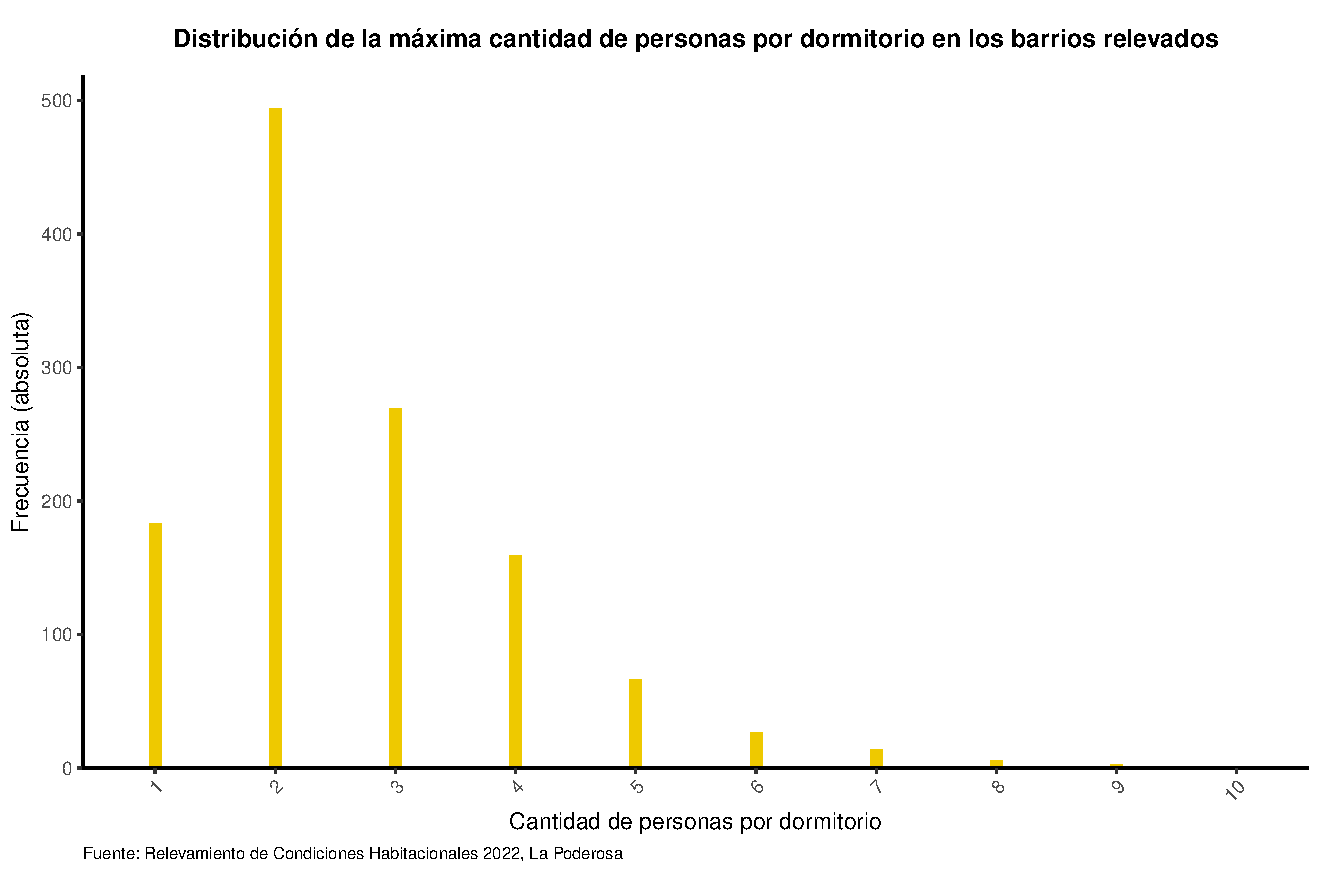
\includegraphics[height=.75\textheight]{graficas-pdf/bastones-hacinamiento.pdf}}
                \only<2>{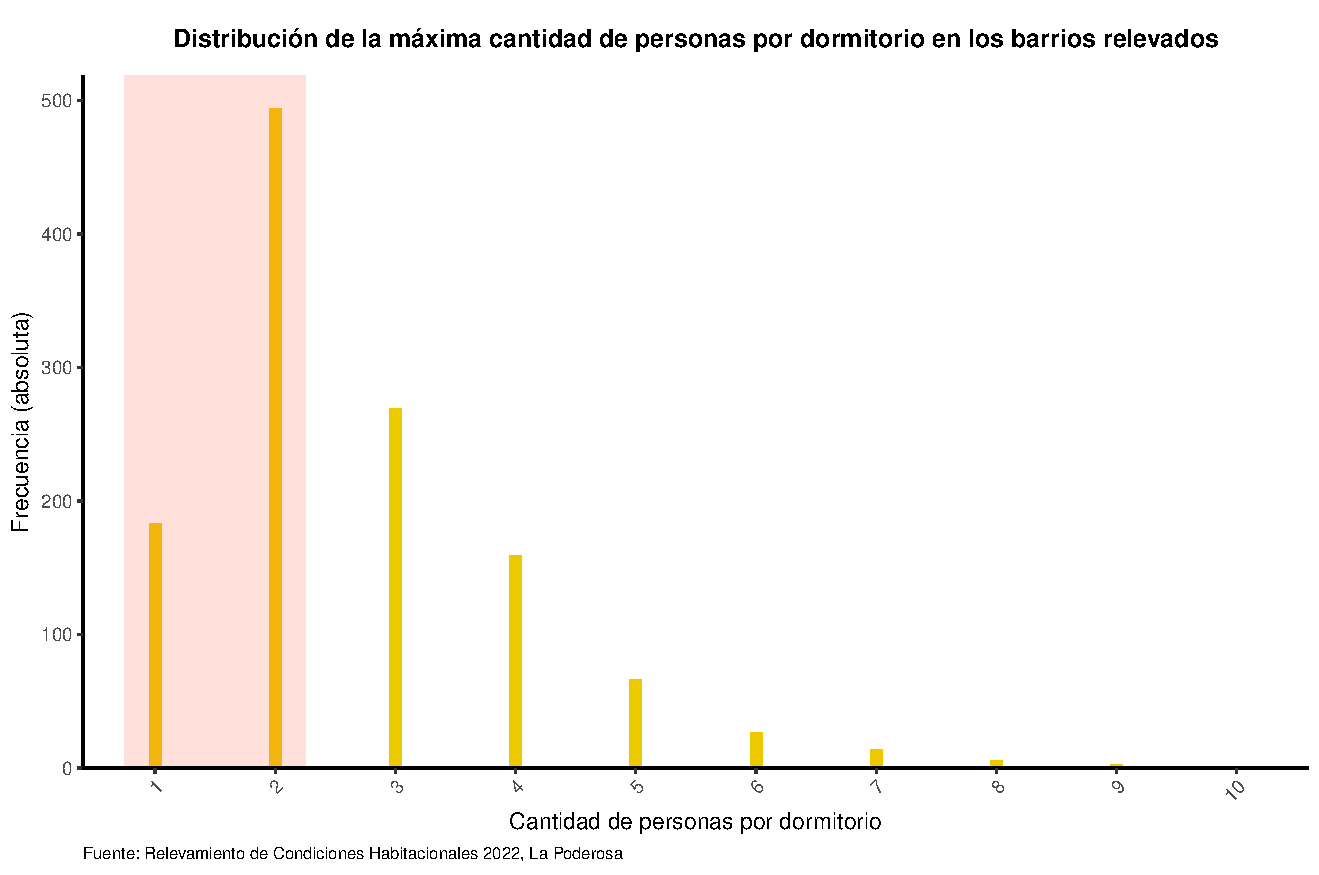
\includegraphics[height=.75\textheight]{graficas-pdf/bastones-hacinamiento-50.pdf}}
                \only<3->{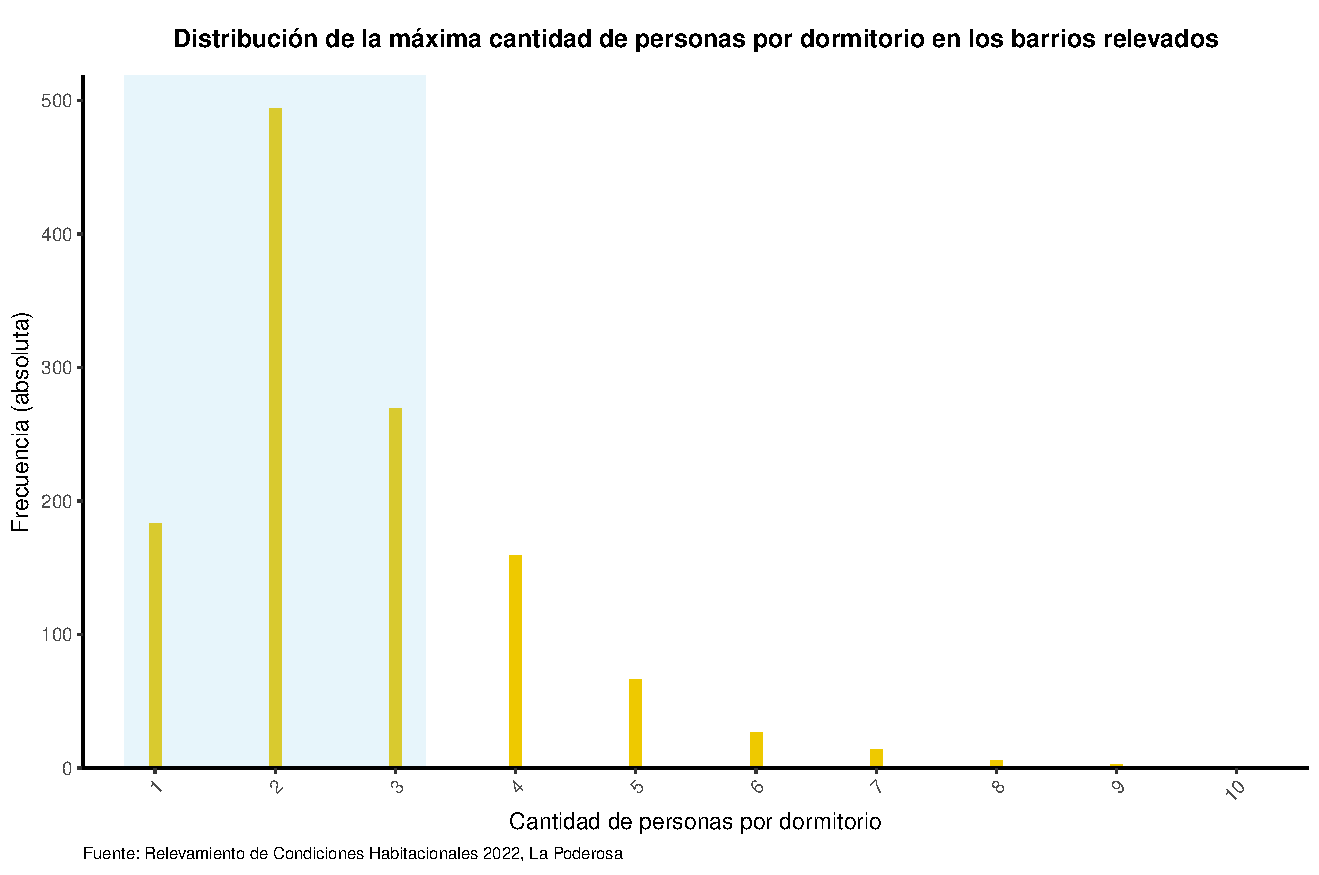
\includegraphics[height=.75\textheight]{graficas-pdf/bastones-hacinamiento-q3.pdf}}
            \end{overlayarea}
        \end{minipage}
        \begin{minipage}{.34\linewidth}
            \setlength{\leftmargini}{12pt}
            \begin{itemize}
                \item<2-> En \textit{más de la mitad} hay \textcolor{tomato}{\textbf{a lo sumo dos} personas} por dormitorio.
                \item<3-> \textit{75\%} reporta un \textcolor{skyblue}{\textbf{máximo de 3 o menos} personas} por habitación. 

                \uncover<4->{O sea, un \textit{25\%} indica tener una habitación con 3 o más personas.}
            \end{itemize}
        \end{minipage}
    \end{frame}

    \begin{frame}{Presión del agua}
        \begin{minipage}{.65\linewidth}
            \begin{overlayarea}{\linewidth}{.75\textheight}
                \only<1>{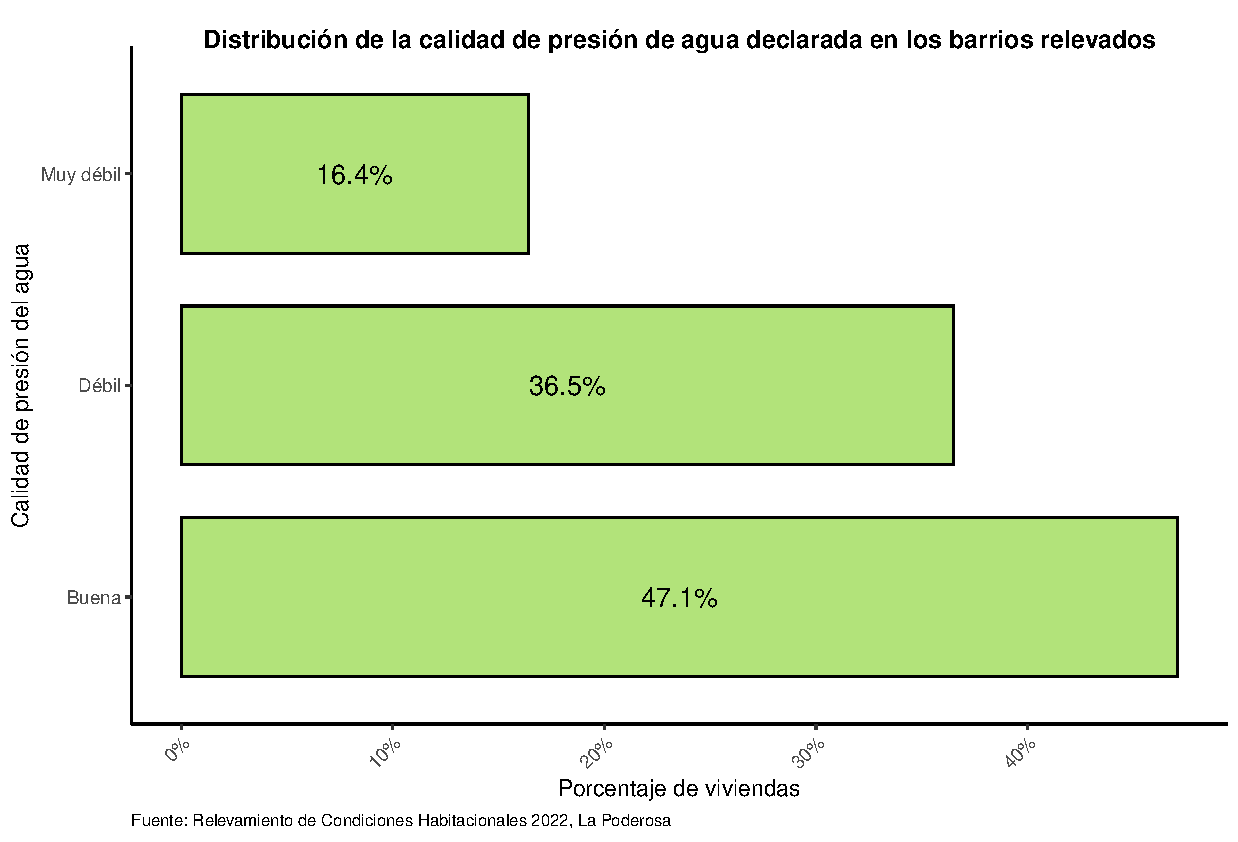
\includegraphics[height=.75\textheight]{graficas-pdf/presion-agua.pdf}}
                \only<2,3>{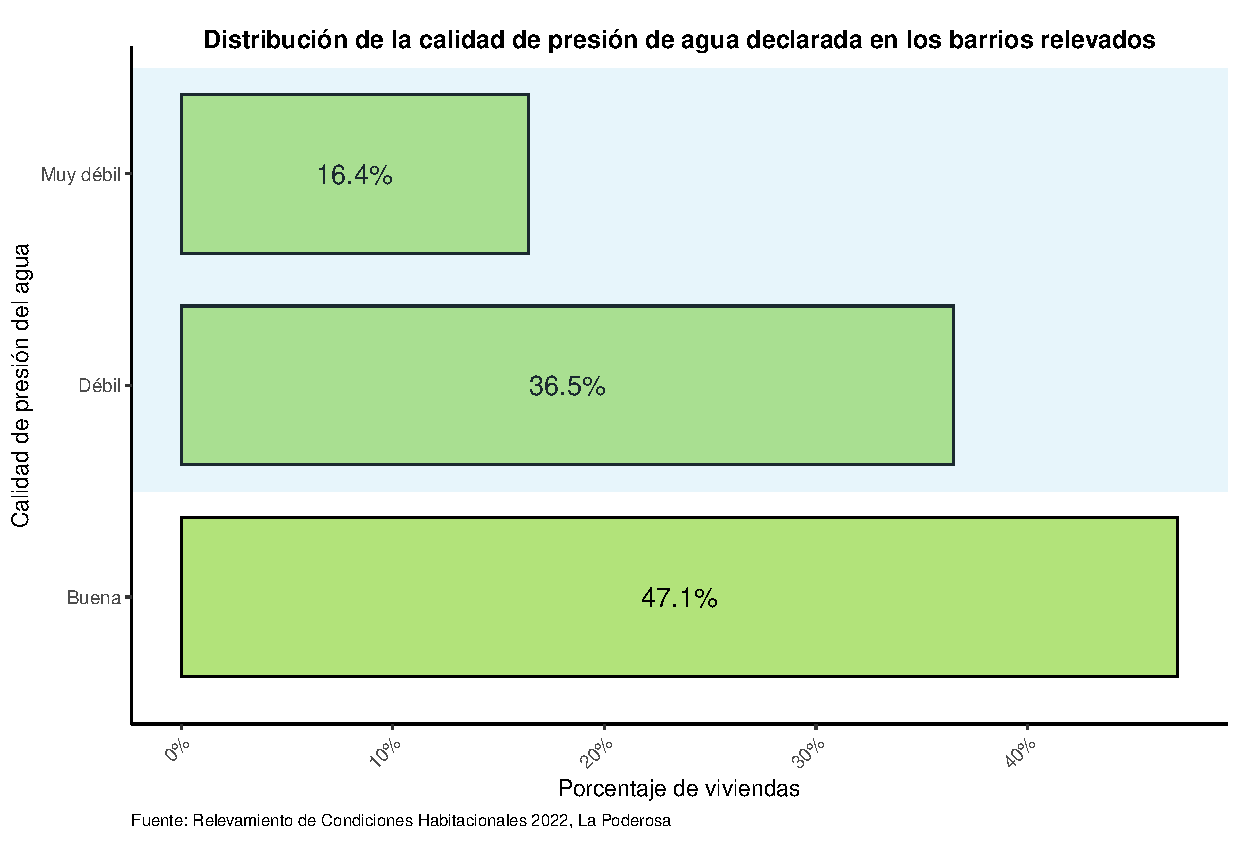
\includegraphics[height=.75\textheight]{graficas-pdf/presion-agua-q2.pdf}}
                \only<4->{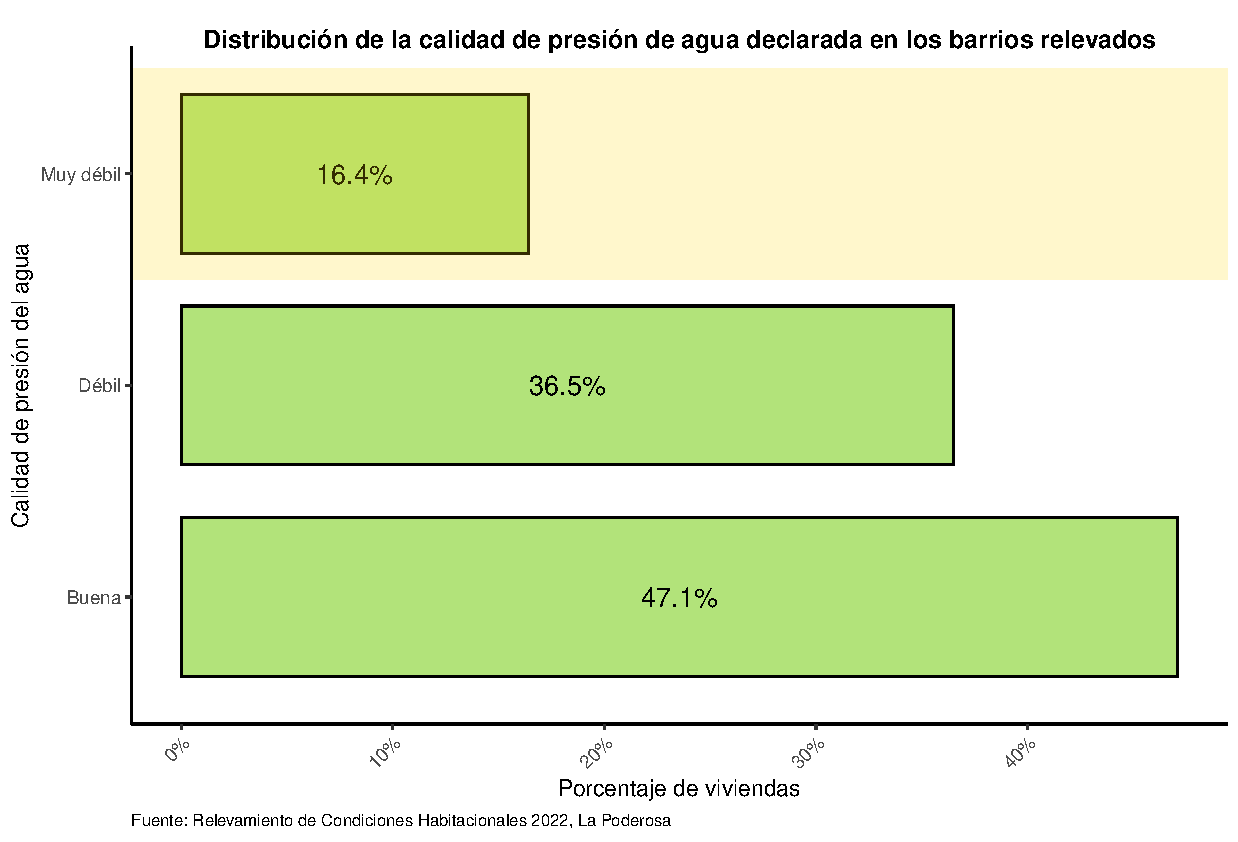
\includegraphics[height=.75\textheight]{graficas-pdf/presion-agua-md.pdf}}
            \end{overlayarea}
        \end{minipage}
        \begin{minipage}{.34\linewidth}
            \setlength{\leftmargini}{12pt}
            \begin{itemize}
                \item<2-> \textit{Más de la mitad} tiene una \textcolor{skyblue}{presión de agua \textbf{débil} o \textbf{muy débil}}. 

                    \uncover<3->{Es decir, en \textit{menos de la mitad} de los hogares la presión es \textbf{buena}.}
                \item<4-> \textit{1 de cada 6} de los hogares relevados presenta \textcolor{gold!90!black}{presión de agua \textbf{muy débil}}.
            \end{itemize}
        \end{minipage}
    \end{frame}
    % TODO: Reordenar diapos para evitar confusiones y más dinámico?

    \begin{frame}{Problemas de humedad por ambiente}
        \begin{minipage}{.65\linewidth}
            \begin{overlayarea}{\linewidth}{.75\textheight}
                \only<1>{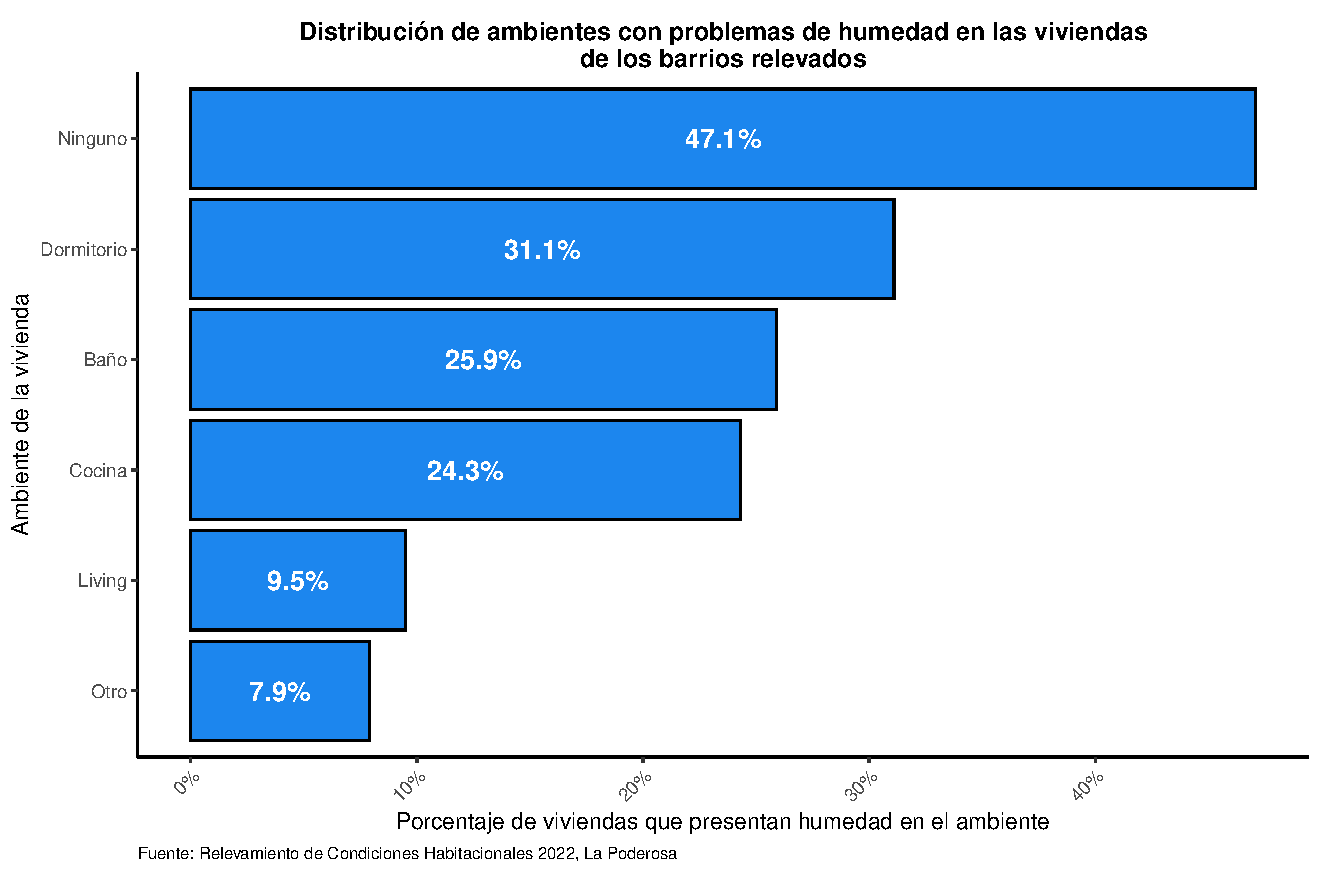
\includegraphics[height=.75\textheight]{graficas-pdf/barras-humedad-horizontal.pdf}}
                \only<2,3>{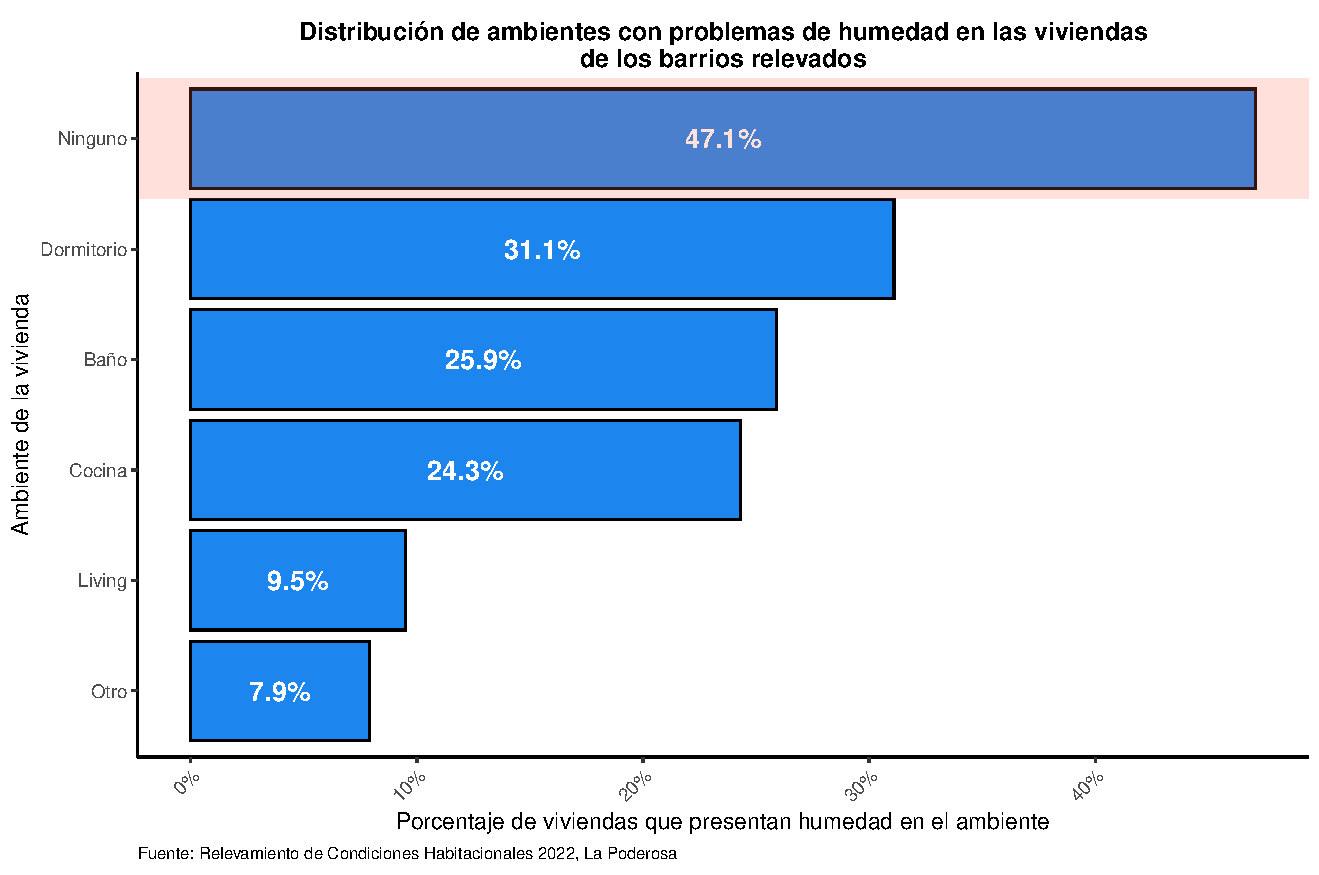
\includegraphics[height=.75\textheight]{graficas-pdf/barras-humedad-horizontal-nh.pdf}}
                \only<4->{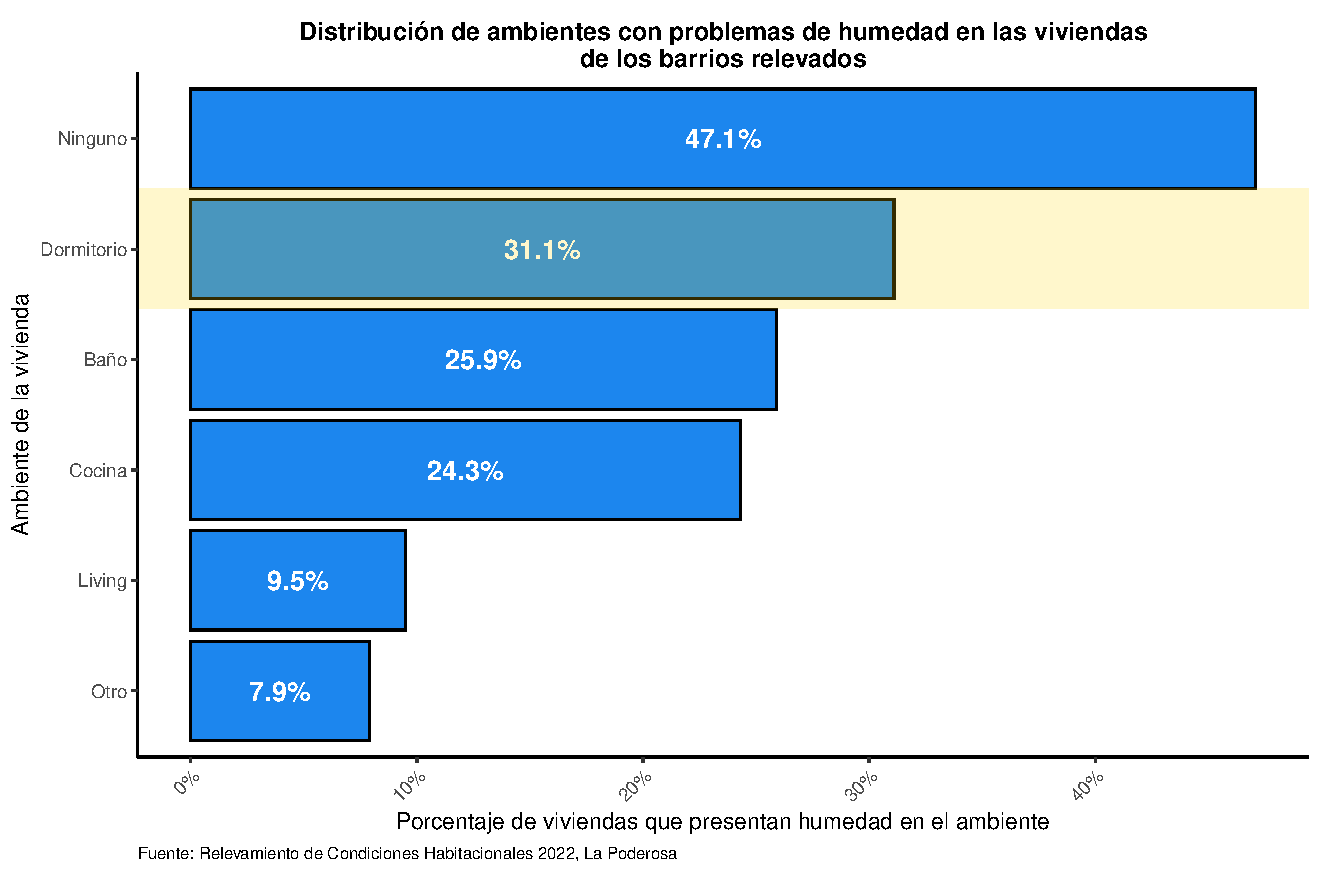
\includegraphics[height=.75\textheight]{graficas-pdf/barras-humedad-horizontal-dorm.pdf}}
            \end{overlayarea}
        \end{minipage}
        \begin{minipage}{.34\linewidth}
            \setlength{\leftmargini}{12pt}
            \begin{itemize}
                \item<2-> \textit{Poco menos del 50\%} \textcolor{tomato}{\textbf{no tienen} problemas de humedad}. 

                    \uncover<3->{Por lo tanto, \textit{más del 50\%} \textbf{sí tiene} problemas de este tipo.}
                \item<4-> Entre las viviendas con problemas de humedad, \textit{la mayoría} \textbf{tiene \textcolor{gold!90!black}{problemas en el dormitorio}}.
            \end{itemize}
        \end{minipage}
    \end{frame}

    \begin{frame}{Calidad del tendido eléctrico}
        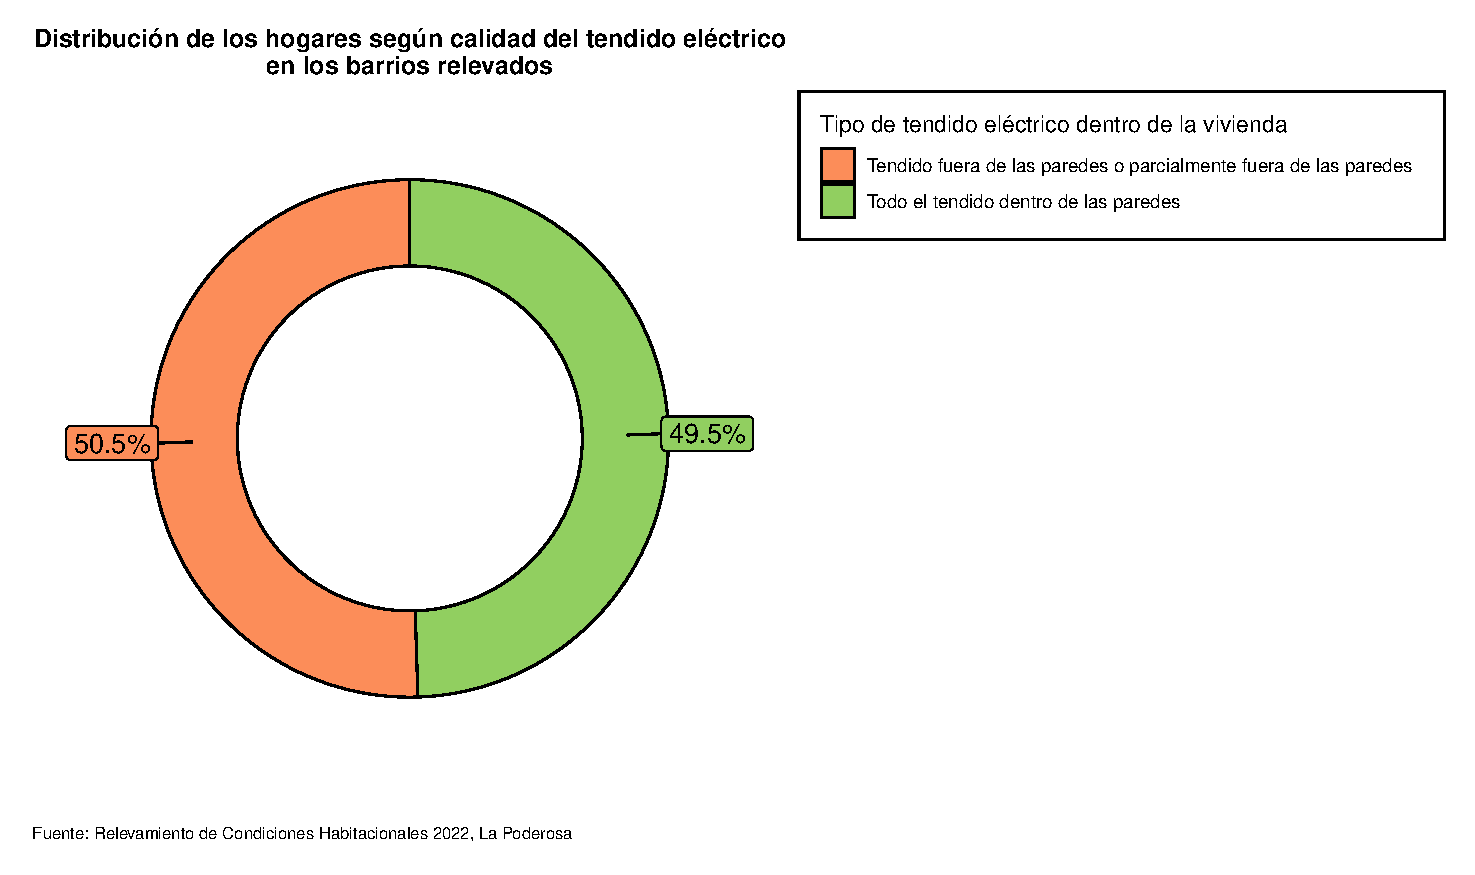
\includegraphics[height=.75\textheight]{graficas-pdf/sectores-circ-calidad-tendido-electrico.pdf}\tikzmark{calidad-tendido}
        \begin{tikzpicture}[overlay, remember picture]
            \coordinate (a) at (pic cs:calidad-tendido);
            \node[text width=9cm, align=left, anchor=north west] at ($ (a) + (-4.75,3.25) $) {\vbox{
                \begin{itemize}
                    \item<2-> \textit{Más de la mitad} de viviendas tienen un tendido eléctrico \textbf{irregular}, con \textcolor{peachorange}{partes o su totalidad \textbf{fuera de las paredes}}.
                \end{itemize}
            }};
        \end{tikzpicture}
    \end{frame}
    
    \section{La importancia del jefe/a del hogar}
    \begin{frame}
        \tableofcontents[currentsection]
    \end{frame} 

    \begin{frame}{Edad del jefe/a del hogar}
         \begin{minipage}{.65\linewidth}
            \begin{overlayarea}{\linewidth}{.75\textheight}
                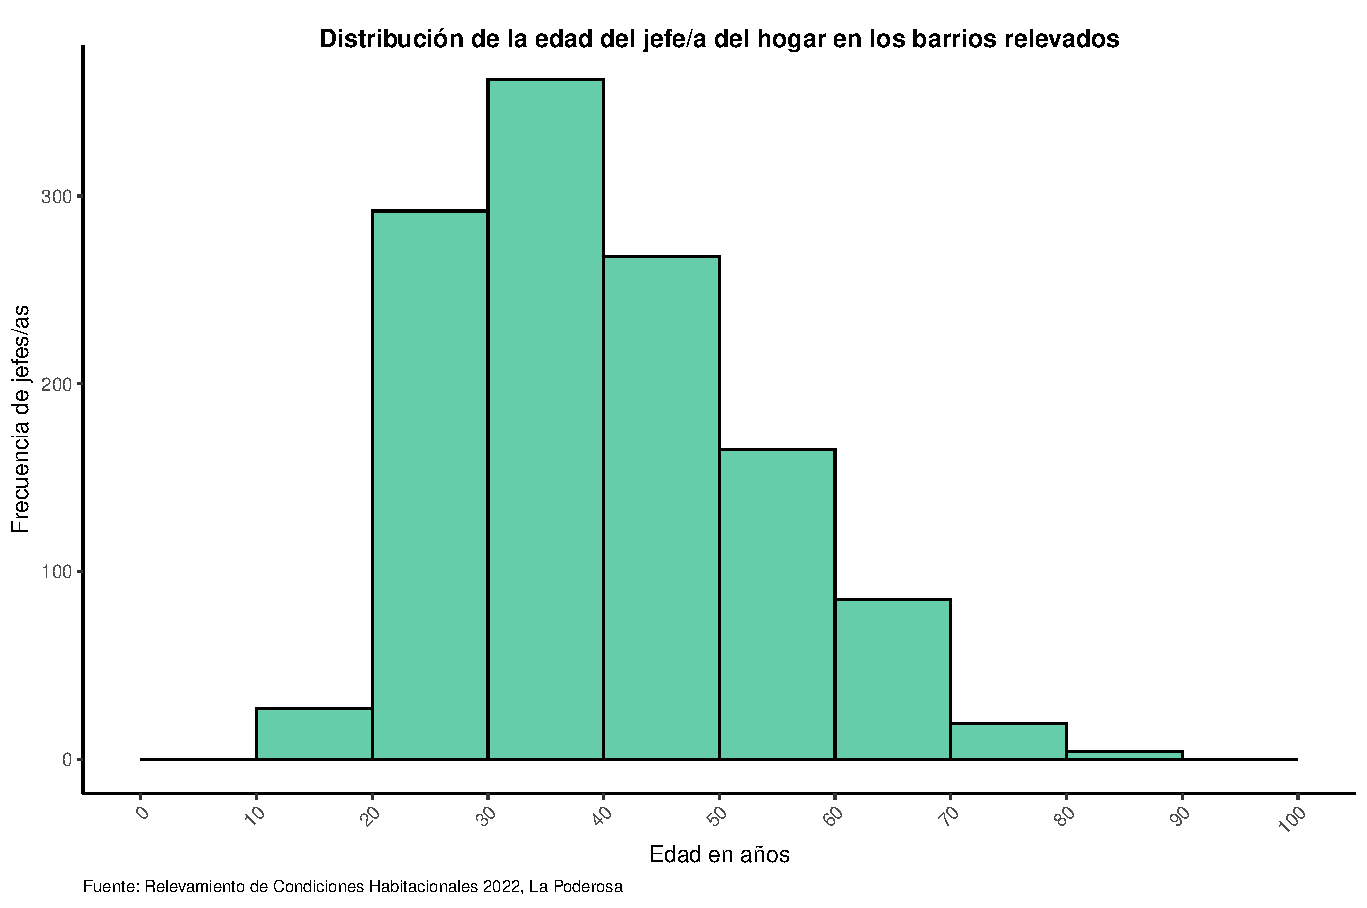
\includegraphics[height=.75\textheight]{graficas-pdf/histograma-edad-jefe.pdf}
            \end{overlayarea}
        \end{minipage}
        \begin{minipage}{.34\linewidth}
            \setlength{\leftmargini}{12pt}
            \begin{itemize}
                \item<2-> Distribución de edades \textit{asimétrica hacia la derecha}.

                \uncover<3->{Edad promedio de 40,4 años, pero \textit{la mitad} tiene \textbf{hasta 38 años} de edad.}
                \item<4-> \textit{El 50\% central} de las edades se encuentra entre \textbf{19-57 años}.

                \uncover<5->{Es decir, \textit{un 25\%} tiene \textbf{hasta 19 años} de edad.}
            \end{itemize}
        \end{minipage}
    \end{frame}

    \begin{frame}{Relación entre edad del jefe/a del hogar y el tiempo de residencia}
         \begin{minipage}{.45\linewidth}
            \begin{overlayarea}{\linewidth}{.75\textheight}
                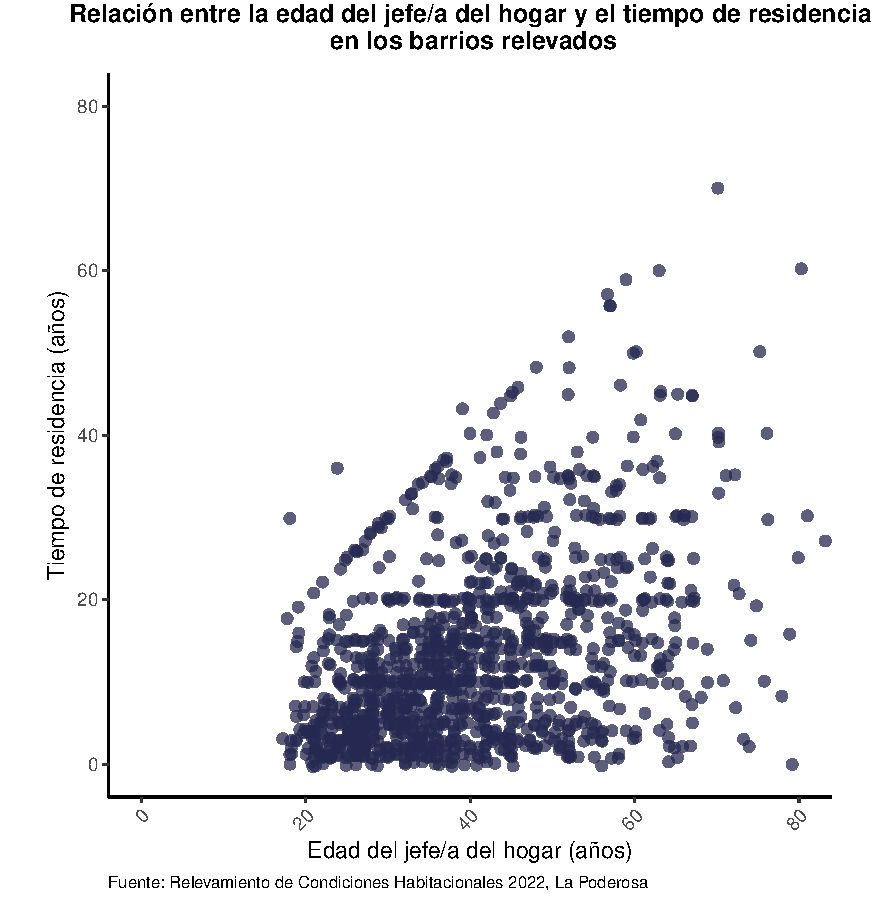
\includegraphics[height=.75\textheight]{graficas-pdf/edad-jefe-tiempo-residencia.pdf}
            \end{overlayarea}
        \end{minipage}
        \begin{minipage}{.54\linewidth}
            \setlength{\leftmargini}{12pt}
            \begin{itemize}
                \item<2-> Más allá de que la edad del jefe/a del hogar suele ser mayor al tiempo de residencia, \textbf{no} se observa ninguna relación significativa entre las variables.
            \end{itemize}
        \end{minipage}
    \end{frame}
    
    \section{Diferencias en la condición de tenencia}
    \begin{frame}
        \tableofcontents[currentsection]
    \end{frame} 

    \begin{frame}{Panorama general de la condición de tenencia}
        \begin{block}{Aclaración}\pause
            Para el propósito del análisis de esta y futuras variables relacionadas a la condición de tenencia, consideraremos que la situación dominial sobre la vivienda es ``Propia'' si en la encuesta original una familia respondió que ``El lugar que habitan actualmente es'':\pause 
            \begin{itemize}
                \item \textit{Propio con algún comprobante de tenencia}
                \item \textit{Propio sin títulos}
            \end{itemize} \pause
            Cualquier otra se considera como que su situación dominial es ``No propia'': \vspace{-8pt} \pause
            \begin{multicols}{2}
                \begin{itemize}
                    \item \textit{Alquilado}
                    \item \textit{Ocupado/Tomado}
                    \item \textit{Prestado}
                    \item \textit{Otro}
                \end{itemize}
            \end{multicols}\vspace{-8pt}
        \end{block}
    \end{frame}

    \begin{frame}{Panorama general de la condición de tenencia (cont.)}
        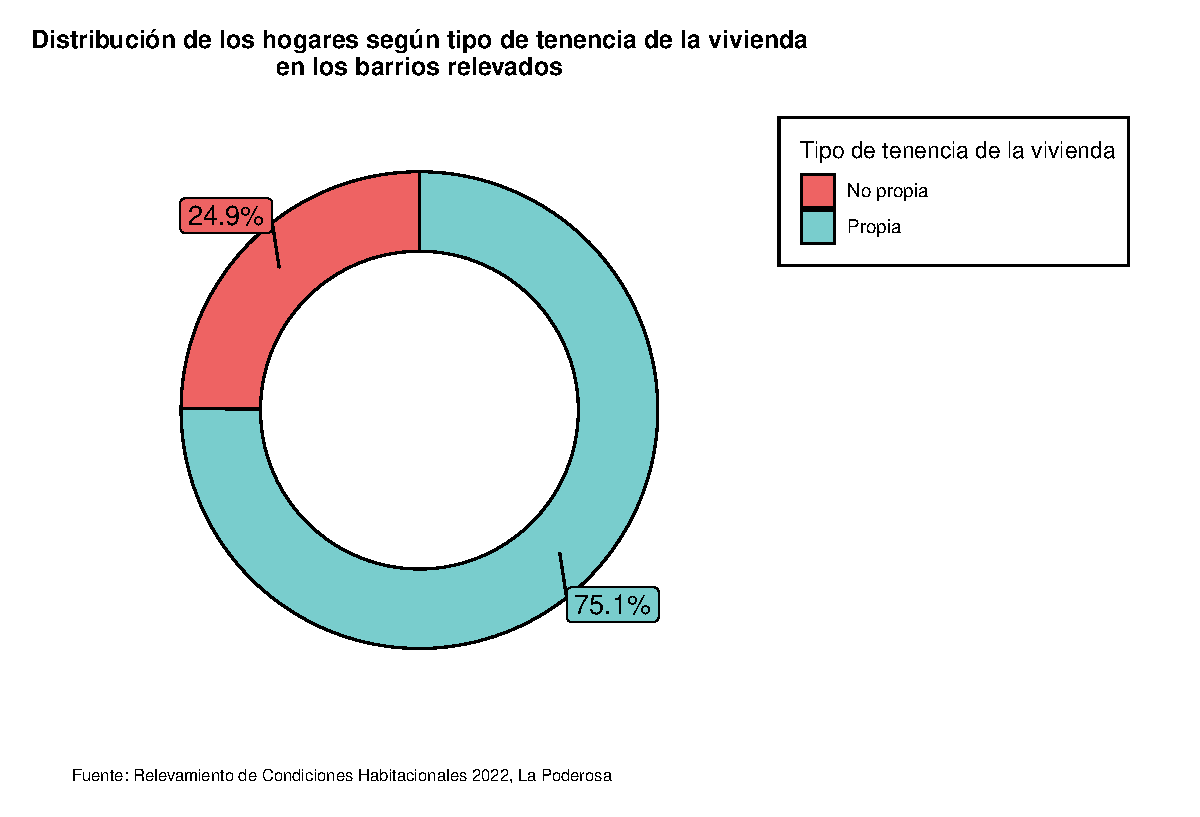
\includegraphics[height=.75\textheight]{graficas-pdf/sectores-circ-tenencia-vivienda.pdf}\tikzmark{tipo-tenencia}
        \begin{tikzpicture}[overlay, remember picture]
            \coordinate (a) at (pic cs:tipo-tenencia);
            \node[text width=8.5cm, align=left, anchor=north west] at ($ (a) + (-3.25,3.25) $) {\vbox{
                \begin{itemize}
                    \item<2-> \textit{Un cuarto} de las viviendas encuestadas \textcolor{indianred2}{\textbf{no pertenecen}} a las familias que las habitan. 
                    \item<3-> Así, los tres cuartos restantes \textcolor{darkslategray3}{\textbf{sí pertenecen}} a sus familias respectivas.
                \end{itemize}
            }};
        \end{tikzpicture}
    \end{frame}
    
    \begin{frame}{Tipos de tenencia por situación dominial \textit{propia} de la vivienda}
        \begin{minipage}{.65\linewidth}
            \begin{overlayarea}{\linewidth}{.75\textheight}
                \only<1>{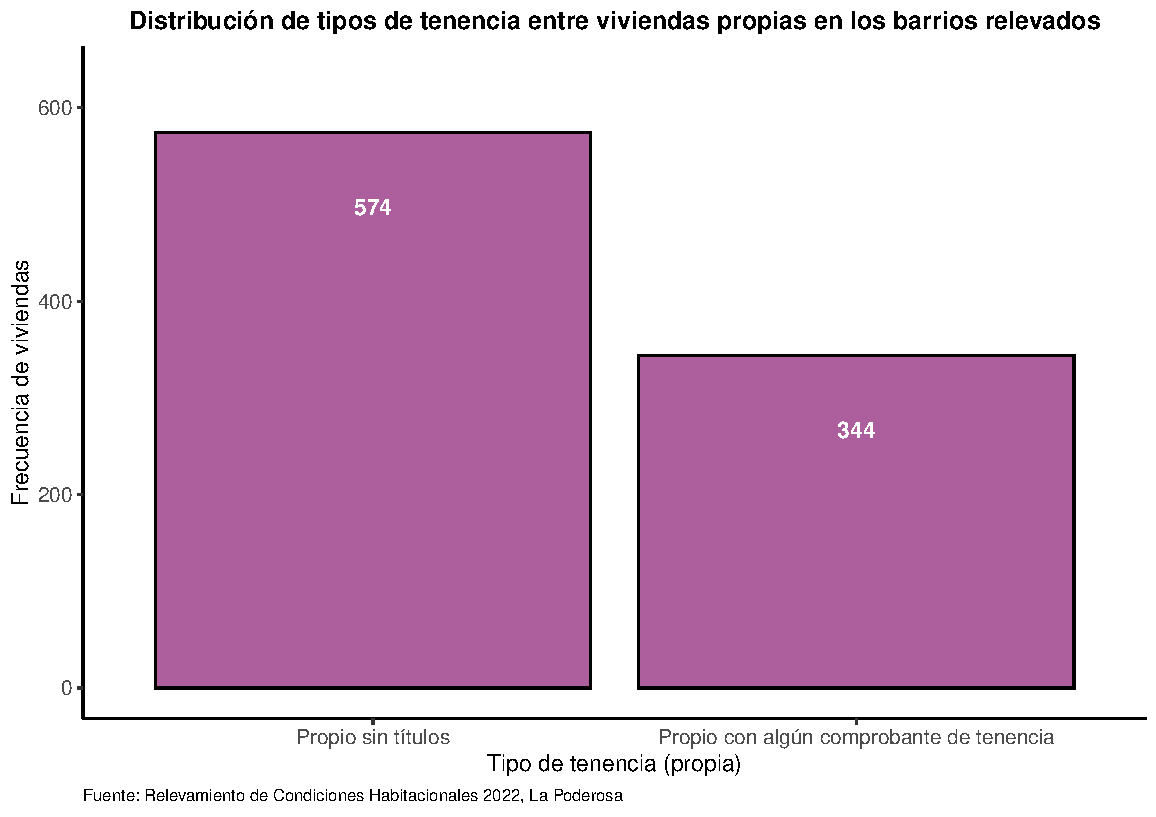
\includegraphics[height=.75\textheight]{graficas-pdf/barras-tipos-tenencia-propia.pdf}}
                \only<2->{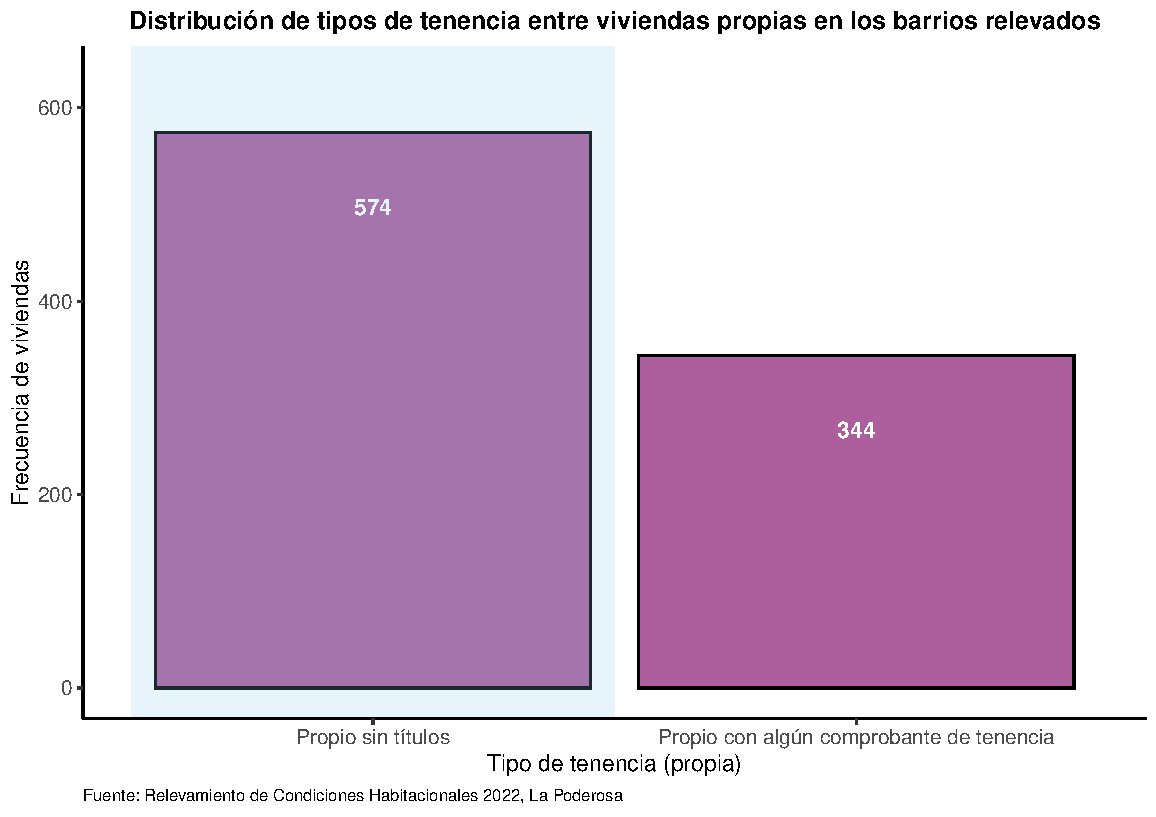
\includegraphics[height=.75\textheight]{graficas-pdf/barras-tipos-tenencia-propia-st.pdf}}
            \end{overlayarea}
        \end{minipage}
        \begin{minipage}{.34\linewidth}
            \setlength{\leftmargini}{12pt}
            \begin{itemize}
                \item<2-> \textit{La mayoría} de las familias encuestadas con tenencia sobre la vivienda \textcolor{skyblue}{\textbf{no tienen} ningún comprobante que lo ratifique}.
            \end{itemize}
        \end{minipage}
    \end{frame}

    \begin{frame}{Tipos de tenencia por situación dominial \textit{no propia} de la vivienda}
        \begin{minipage}{.65\linewidth}
            \begin{overlayarea}{\linewidth}{.75\textheight}
                \only<1>{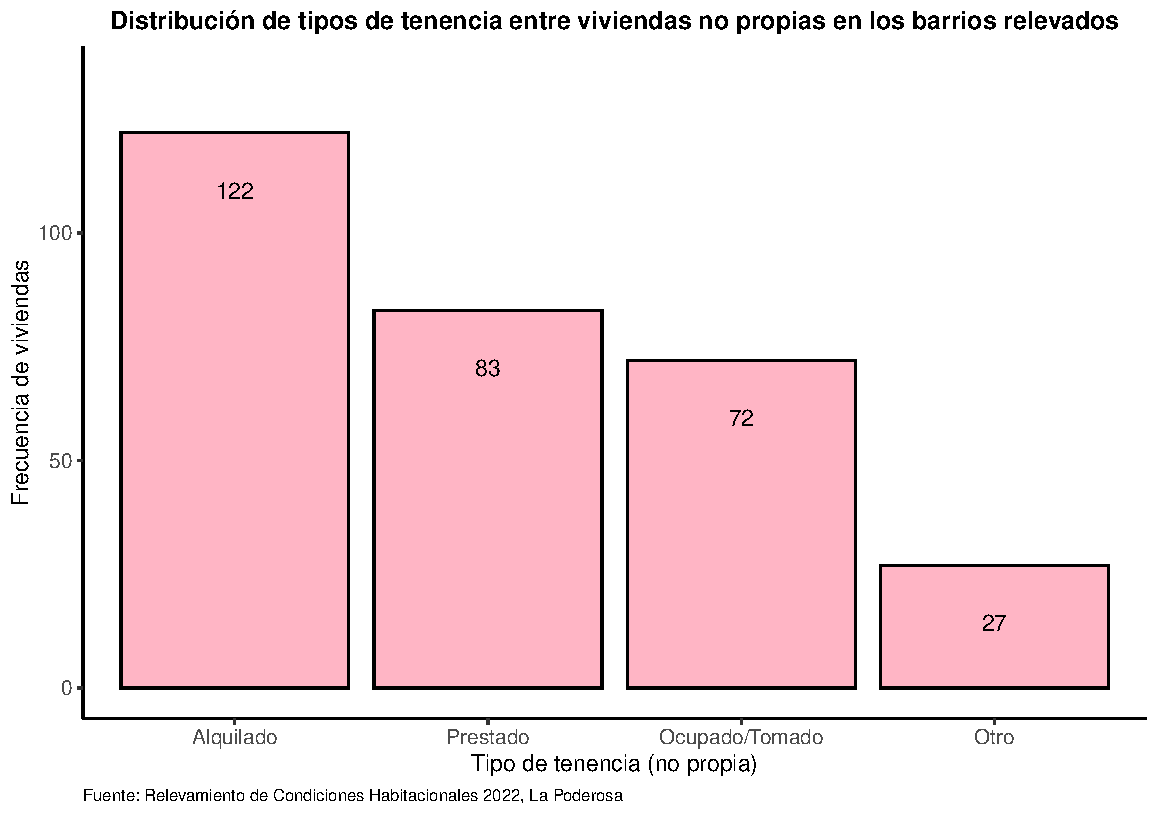
\includegraphics[height=.75\textheight]{graficas-pdf/barras-tipos-tenencia-no-propia.pdf}}
                \only<2->{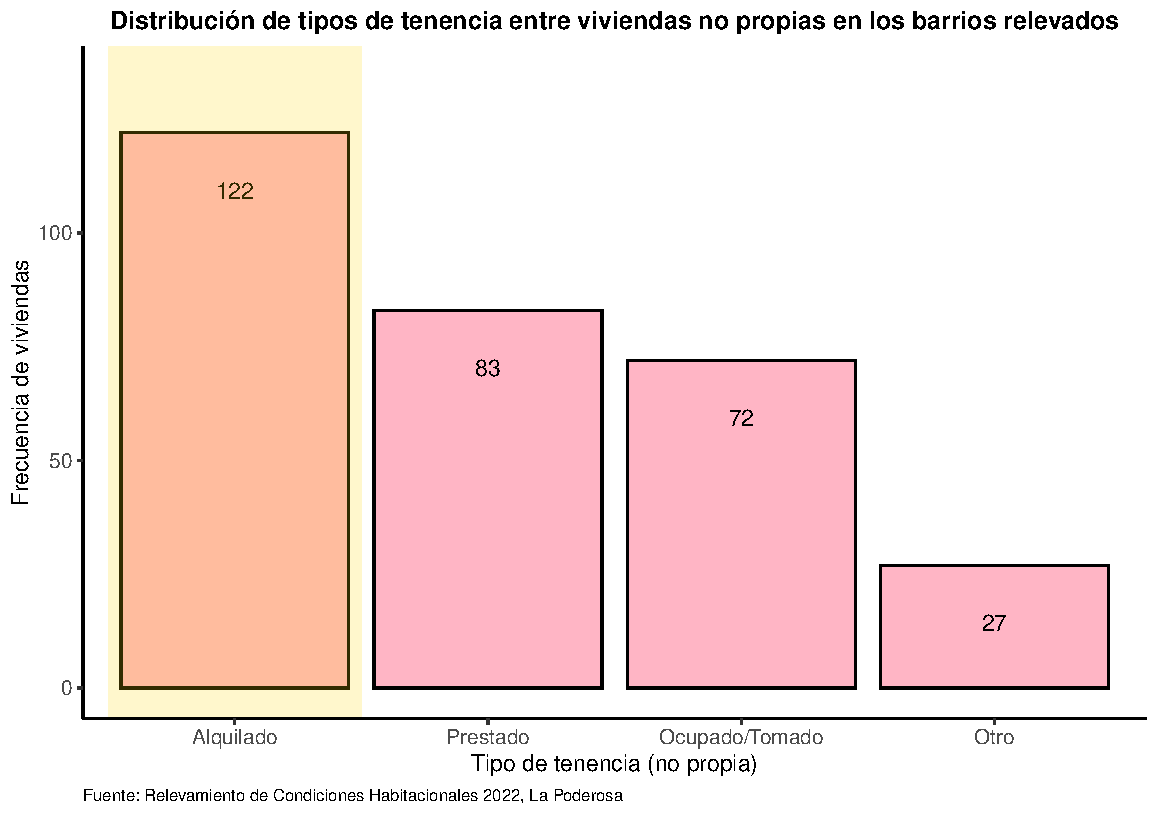
\includegraphics[height=.75\textheight]{graficas-pdf/barras-tipos-tenencia-no-propia-alq.pdf}}
            \end{overlayarea}
        \end{minipage}
        \begin{minipage}{.34\linewidth}
            \setlength{\leftmargini}{12pt}
            \begin{itemize}
                \item<2-> Entre las familias encuestadas sin tenencia sobre la vivienda, \textit{el grupo más numeroso} es el de aquellas que \textbf{\textcolor{gold!90!black}{alquilan}}.
            \end{itemize}
        \end{minipage}
    \end{frame}

    \begin{frame}{Costo del alquiler}
        \begin{minipage}{.65\linewidth}
            \begin{overlayarea}{\linewidth}{.75\textheight}
                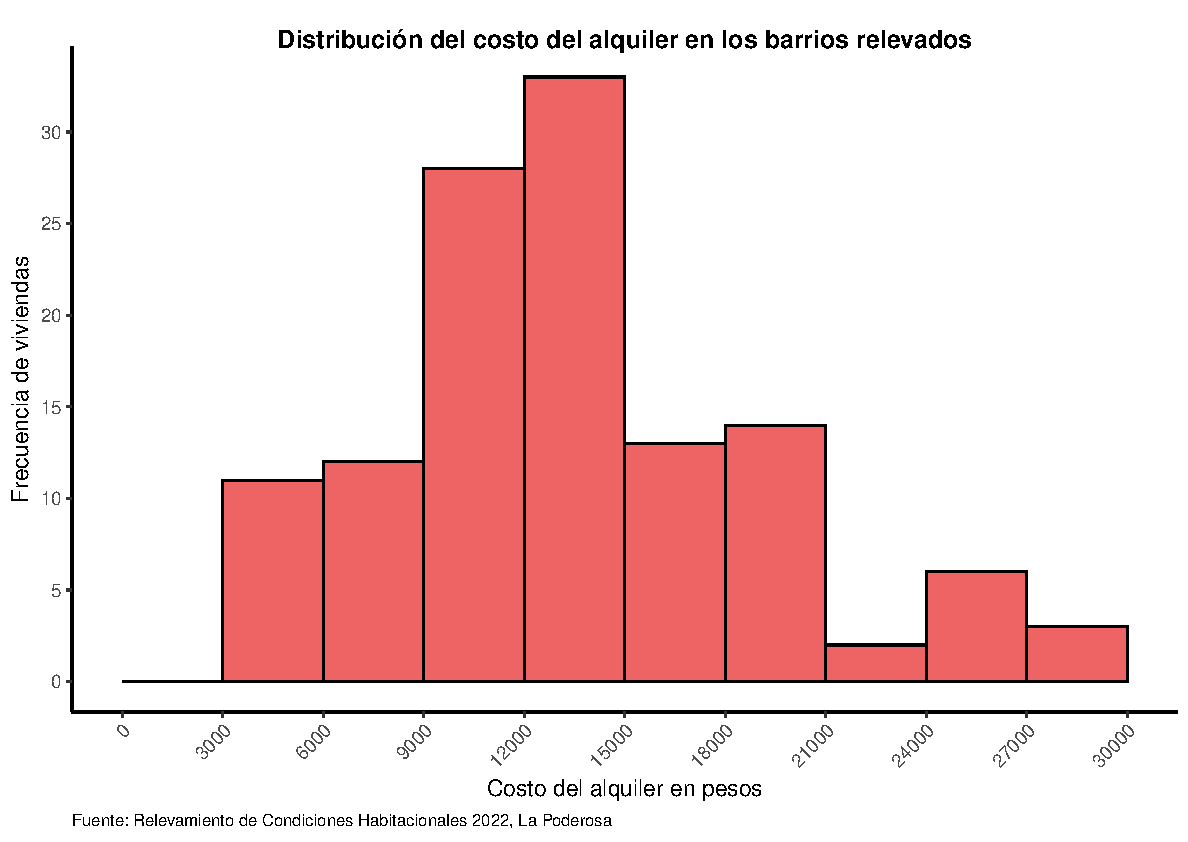
\includegraphics[height=.75\textheight]{graficas-pdf/histograma-costo-alquiler.pdf}
            \end{overlayarea}
        \end{minipage}
        \begin{minipage}{.34\linewidth}
            \small
            \setlength{\leftmargini}{8pt}
            \begin{itemize}
                \item<2-> Precios en el intervalo \textbf{3500-30000 pesos}.
                \item<3-> Distribución \textit{bastante simétrica}, aunque se observan levemente más registros hacia valores más elevados.
                \item<4-> Precio promedio de \textbf{alrededor de 14000 pesos}.

                    \uncover<5->{\textit{Moderada concentración de valores} en torno a este valor, en un \textbf{intervalo de aproximadamente 5000 pesos}.}
            \end{itemize}
        \end{minipage}
    \end{frame}

    \begin{frame}{Relación entre edad del jefe/a del hogar y la condición de tenencia}
        \begin{minipage}{.65\linewidth}
            \begin{overlayarea}{\linewidth}{.75\textheight}
                \only<1-2>{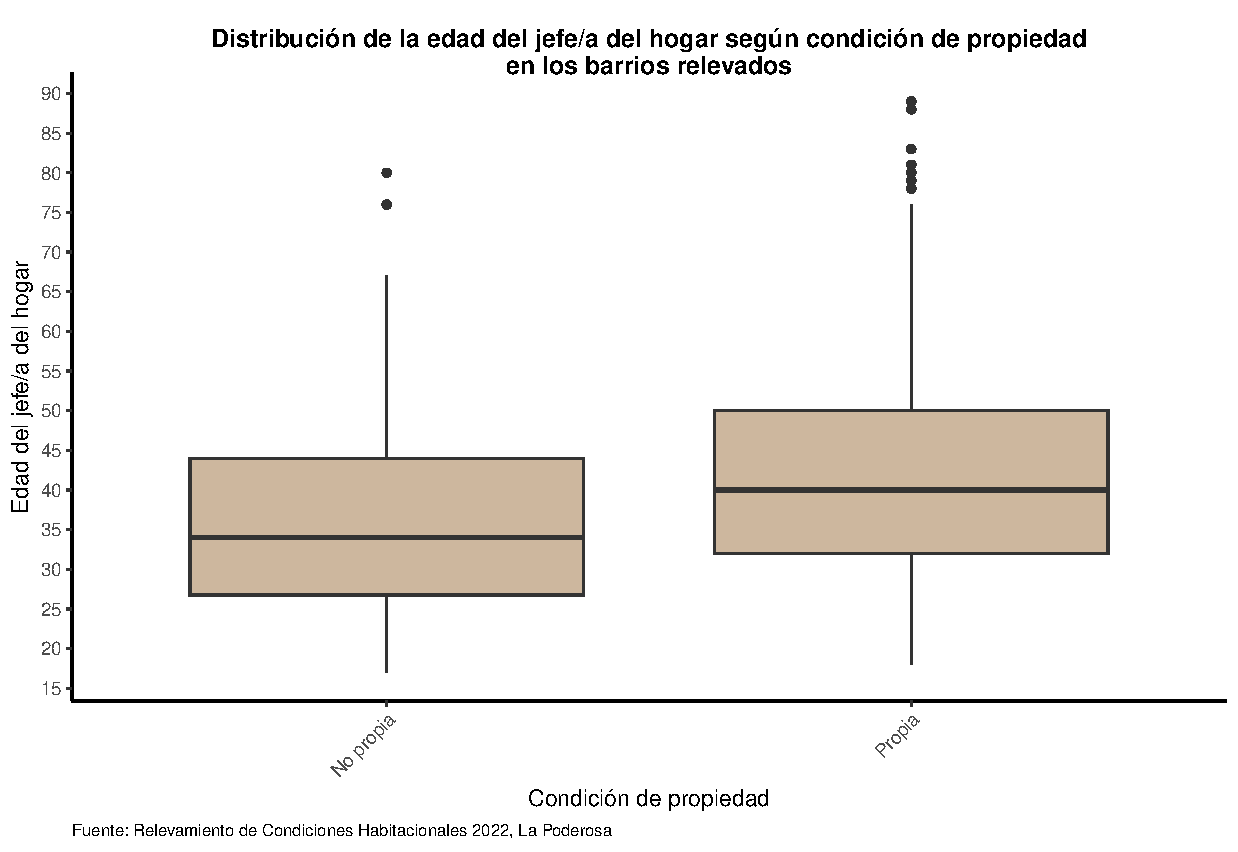
\includegraphics[height=.75\textheight]{graficas-pdf/boxplot-edad-jefe-propiedad.pdf}}
                \only<3>{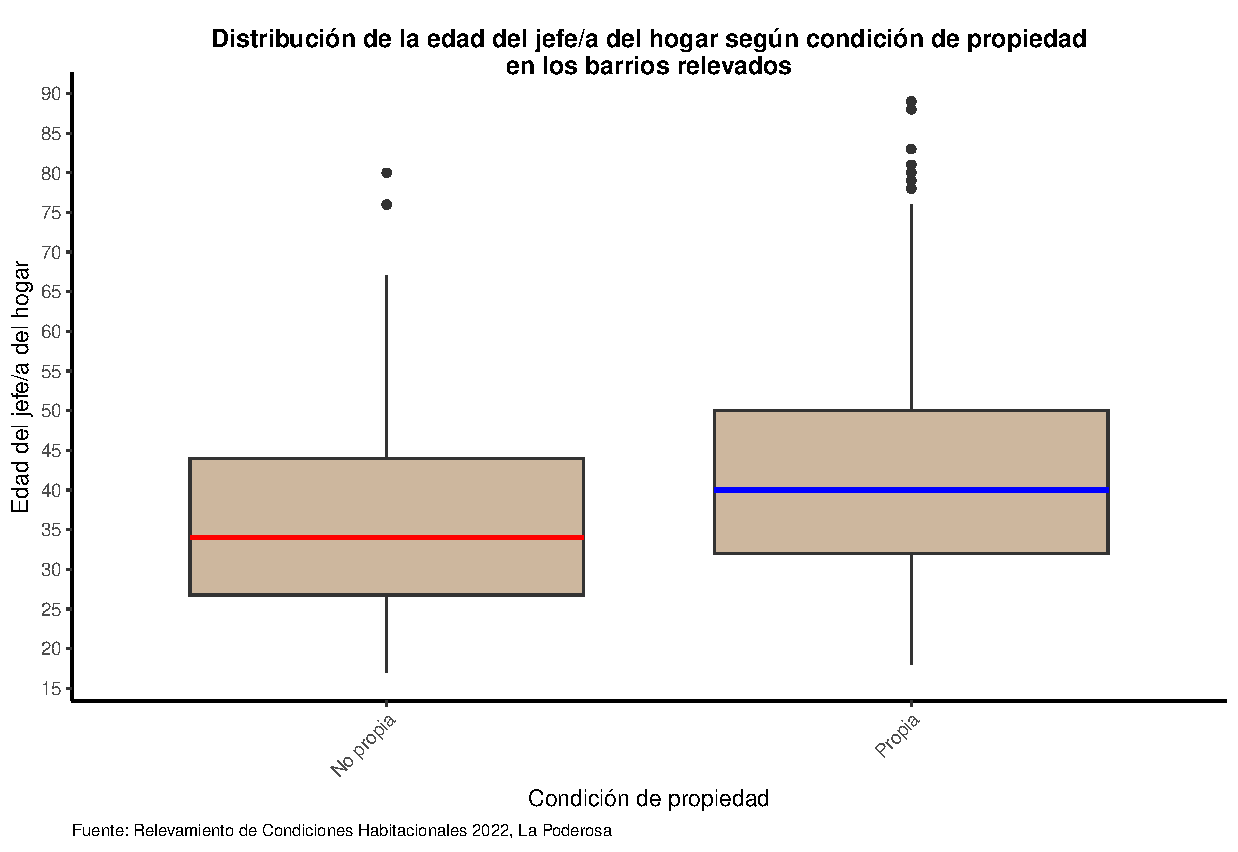
\includegraphics[height=.75\textheight]{graficas-pdf/boxplot-edad-jefe-propiedad-med.pdf}}
                \only<4->{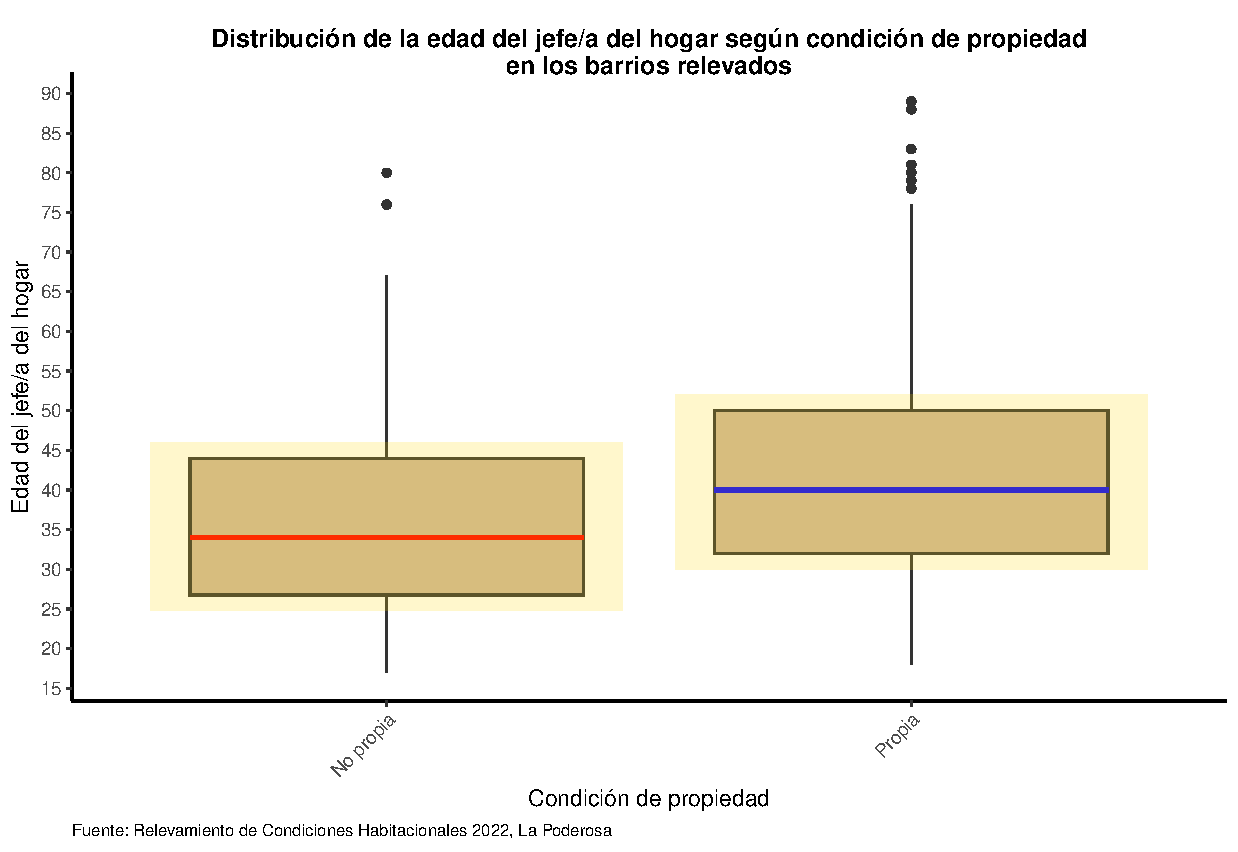
\includegraphics[height=.75\textheight]{graficas-pdf/boxplot-edad-jefe-propiedad-med-ri.pdf}}
            \end{overlayarea}
        \end{minipage}
        \begin{minipage}{.34\linewidth}
            \small
            \setlength{\leftmargini}{8pt}
            \begin{itemize}
                \item<2-> \textbf{Rango etario similar}, aunque con mayor cantidad de \textit{edades mayores} registradas en viviendas propias.
                \item<3-> \textit{Edad central} en \textcolor{red}{viviendas no propias de \textbf{34 años}}, y en \textcolor{blue}{propias de \textbf{40 años}}.
                \item<4-> La mitad de las edades relevadas se concentran de \textit{forma similar} en ambos casos alrededor a la edad central, en un \textcolor{gold!90!black}{\textbf{intervalo de aproximadamente 18 años}}.
            \end{itemize}
        \end{minipage}
    \end{frame}

    \begin{frame}{Relación entre el tiempo de residencia y la condición de tenencia}
        \begin{minipage}{.60\linewidth}
            \begin{overlayarea}{\linewidth}{.85\textheight}
                \only<1-3>{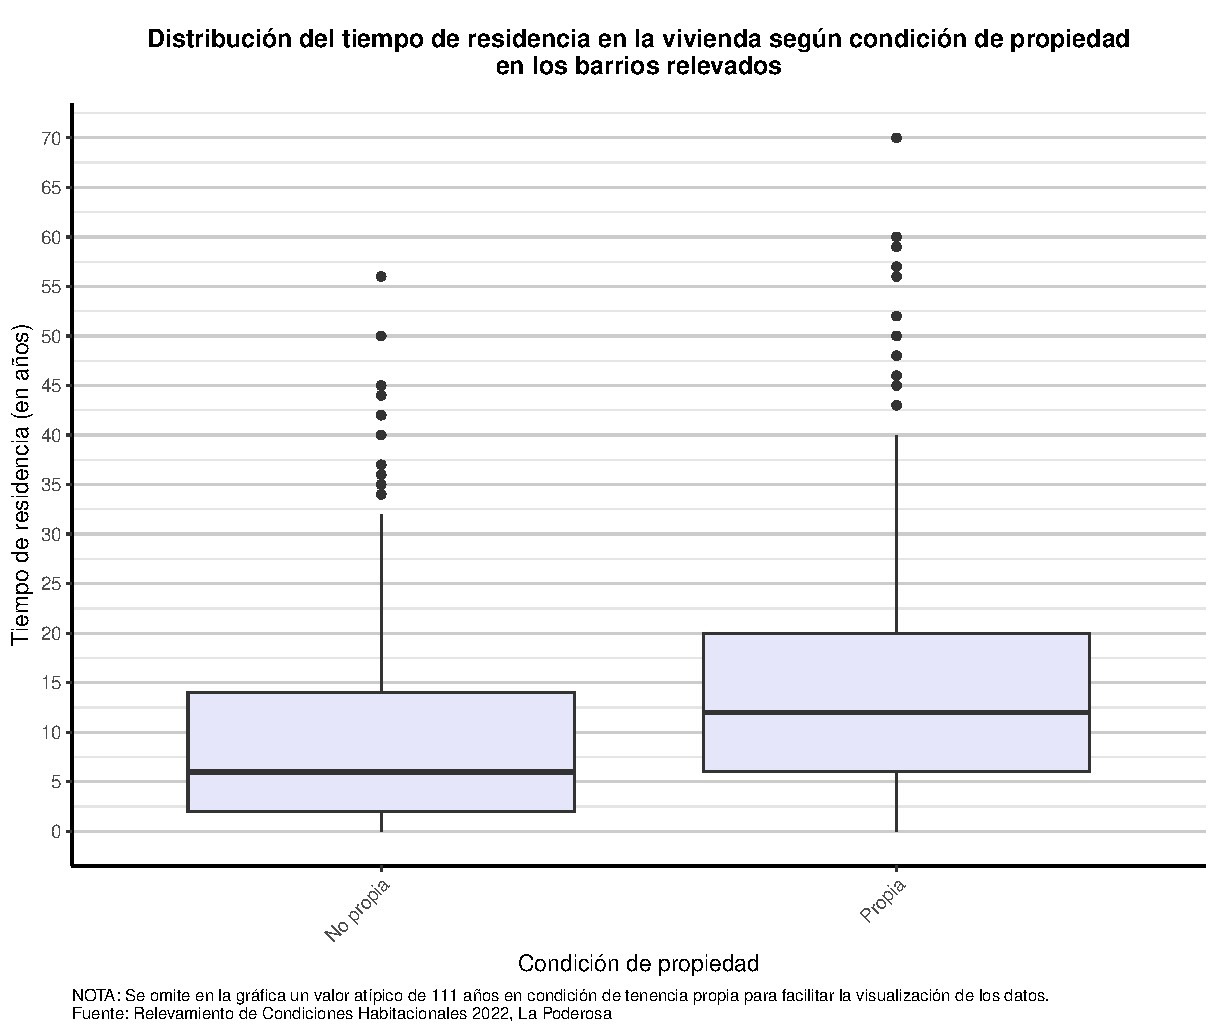
\includegraphics[height=.85\textheight]{graficas-pdf/boxplot-residencia-propiedad-sinatipico.pdf}}
                \only<4->{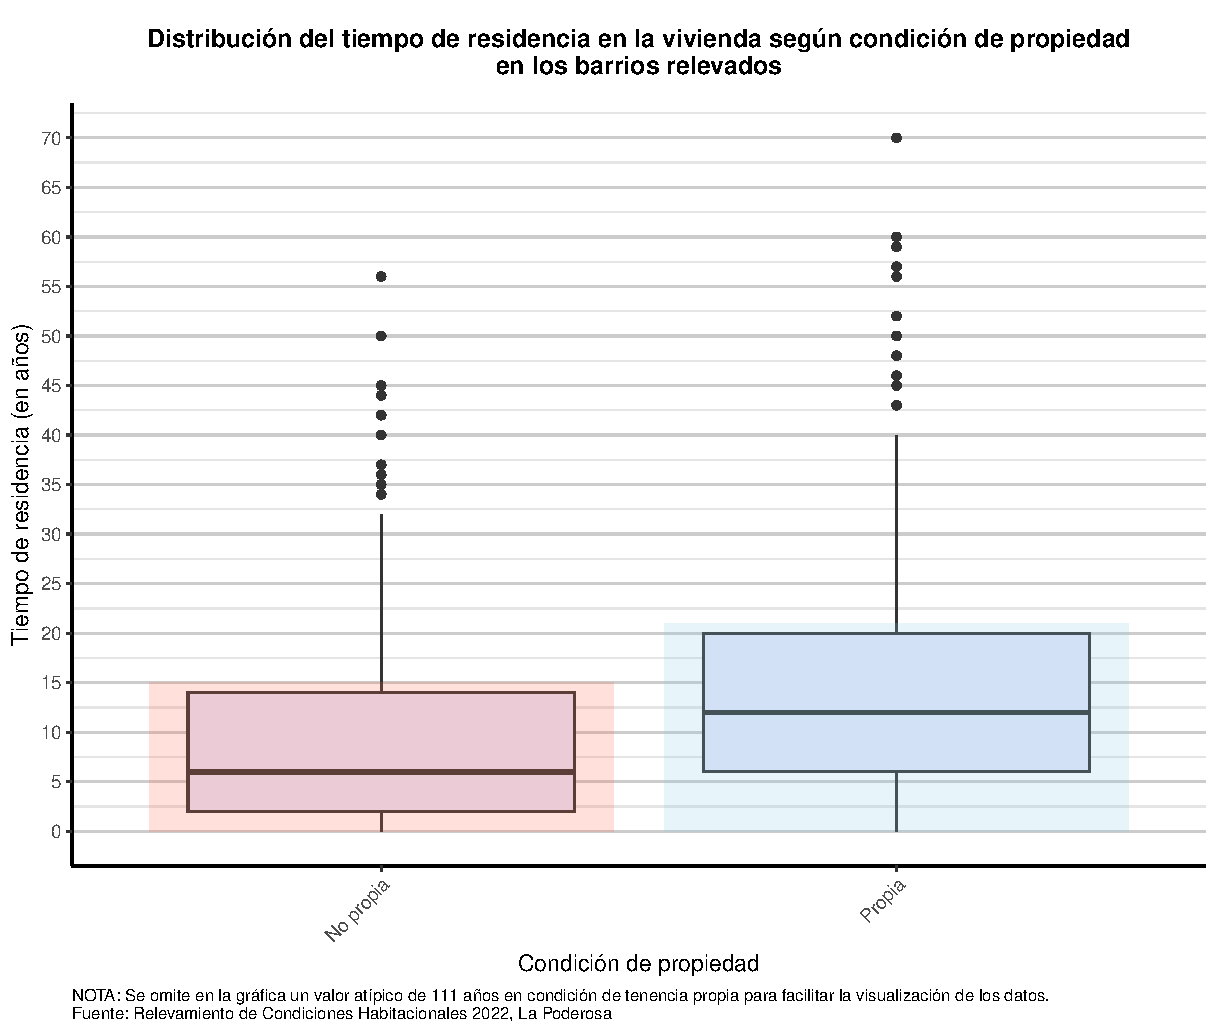
\includegraphics[height=.85\textheight]{graficas-pdf/boxplot-residencia-propiedad-sinatipico-q3.pdf}}
            \end{overlayarea}
        \end{minipage}
        \begin{minipage}{.39\linewidth}
            \small
            \setlength{\leftmargini}{8pt}
            \begin{itemize}
                \item<2-> Tiempo de residencia \textbf{levemente más prolongado} en \textit{viviendas propias}, con un promedio de \textbf{5 años} mayor a las viviendas no propias \uncover<3->{(9,9 años contra 14,2 años).}

                \item<4-> \textit{3 de cada 4 familias} en hogares no propios tienen un \textcolor{tomato}{tiempo de residencia \textbf{menor a los 15 años}}, mientras que este número incrementa a \textcolor{skyblue}{\textbf{menor a 20 años}} para los propios.
            \end{itemize}
        \end{minipage}
    \end{frame}
    
    \begin{frame}{Tiempo de residencia en viviendas \textit{no propias}}
        \begin{minipage}{.65\linewidth}
            \begin{overlayarea}{\linewidth}{.85\textheight}
                \only<1>{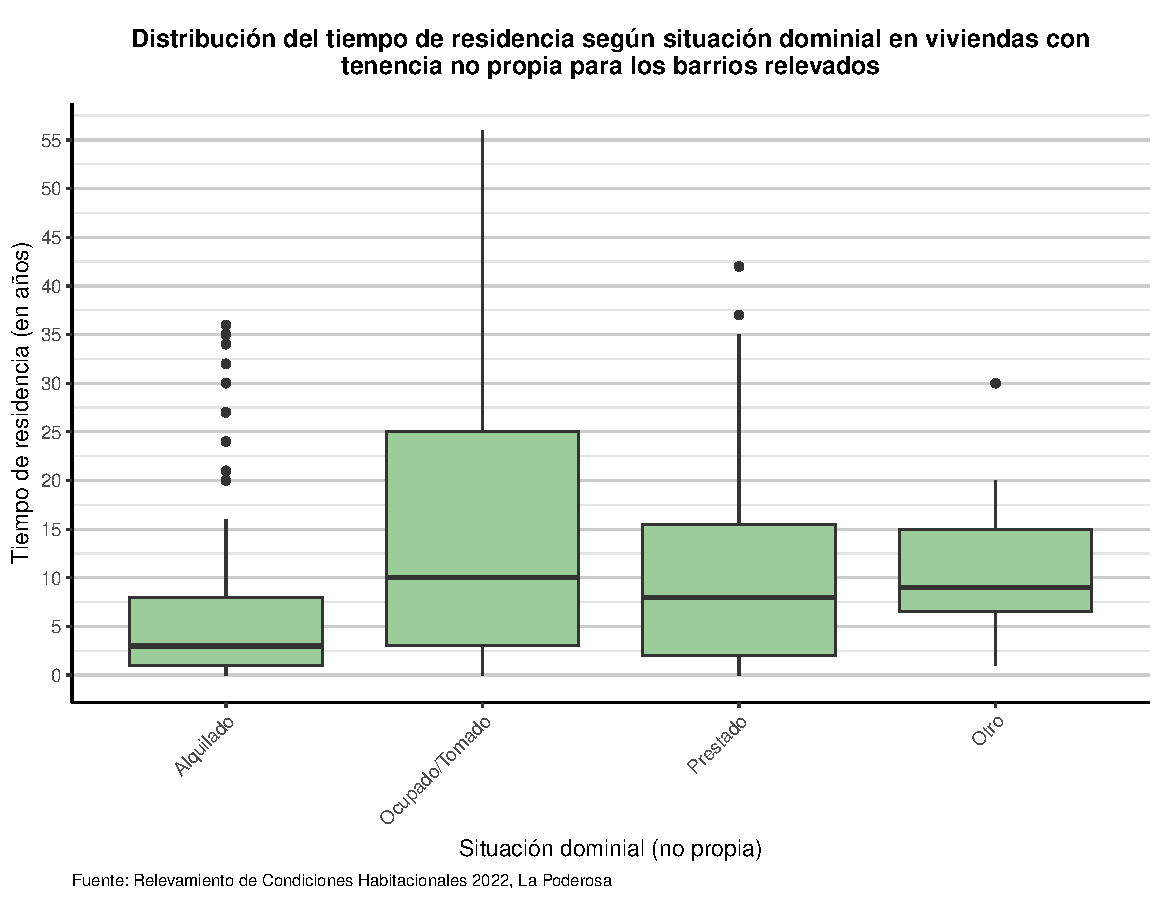
\includegraphics[height=.85\textheight]{graficas-pdf/boxplot-residencia-nopropia-multivariado.pdf}}
                \only<2>{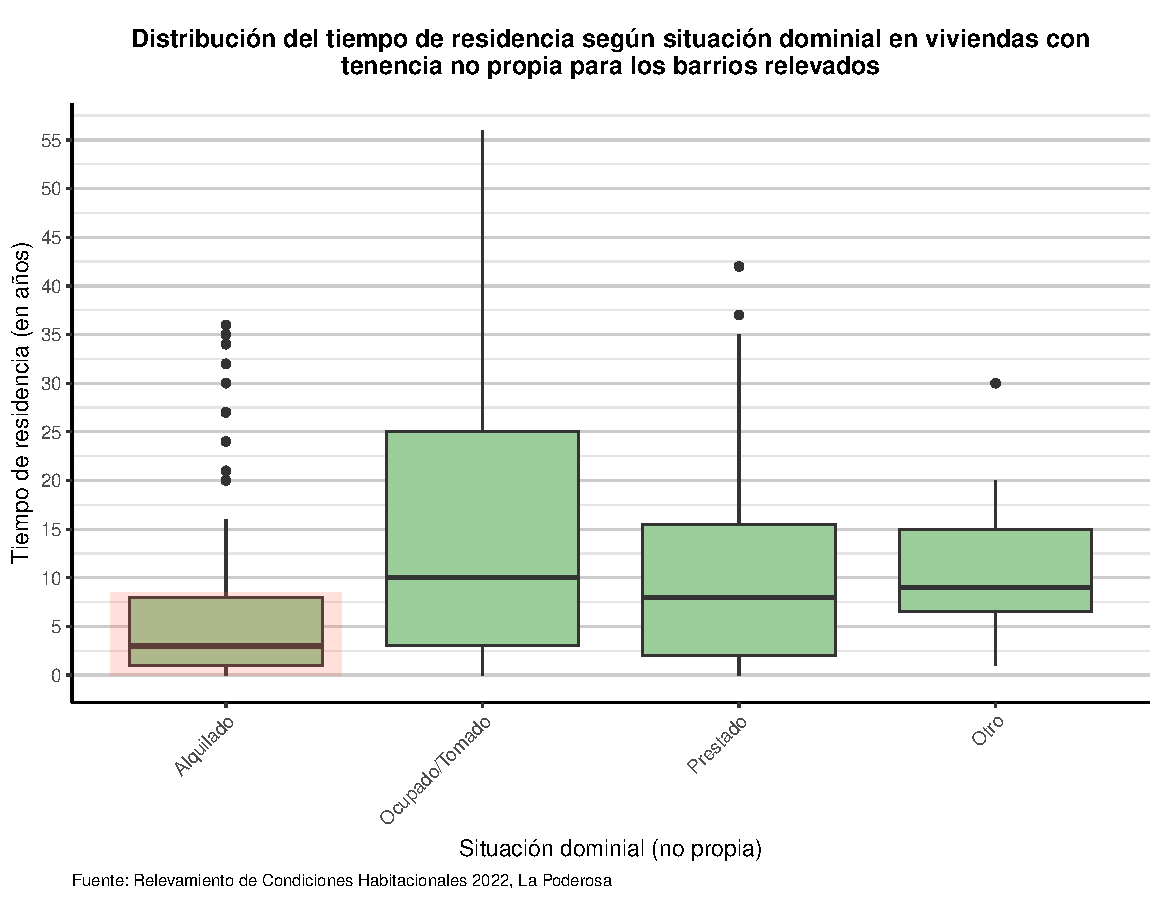
\includegraphics[height=.85\textheight]{graficas-pdf/boxplot-residencia-nopropia-multivariado-alq-q3.pdf}}
                \only<3>{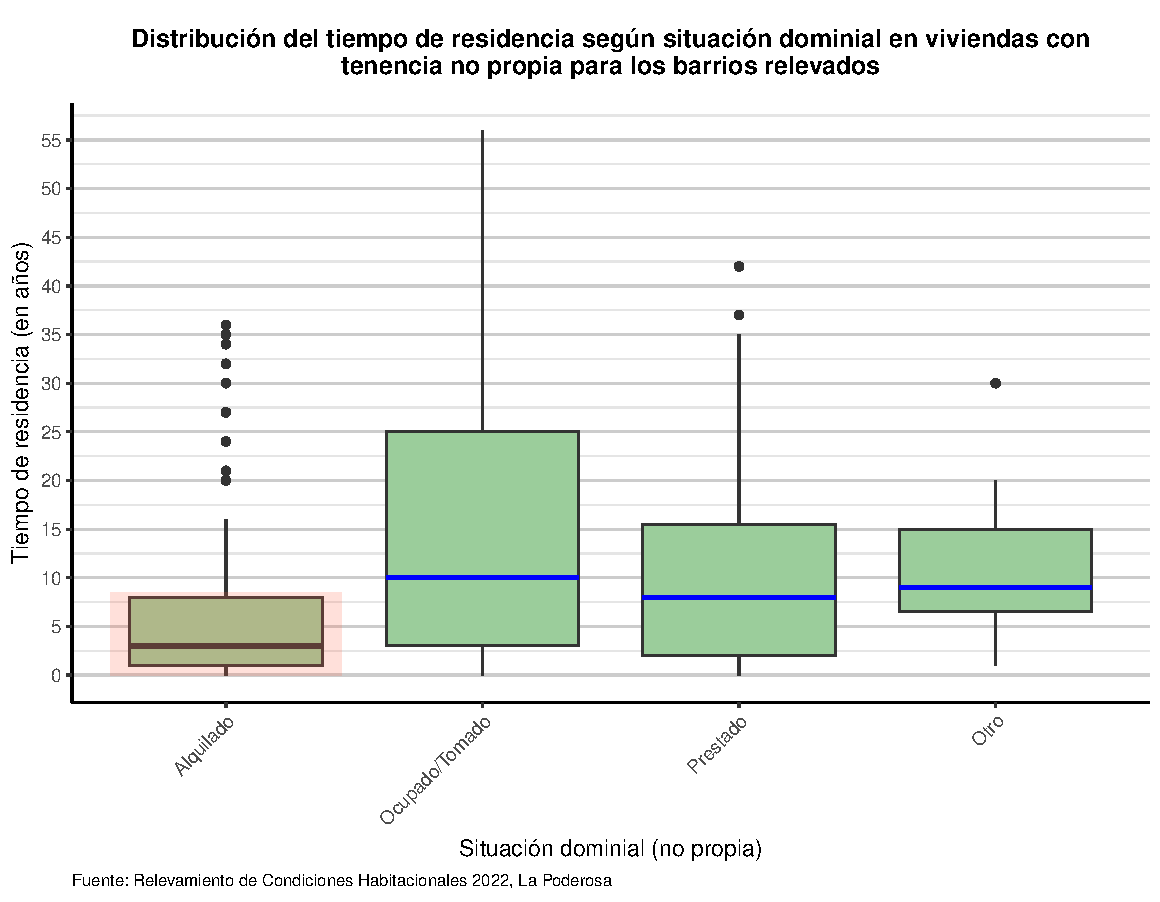
\includegraphics[height=.85\textheight]{graficas-pdf/boxplot-residencia-nopropia-multivariado-alq-q3-med.pdf}}
            \end{overlayarea}
        \end{minipage}
        \begin{minipage}{.34\linewidth}
            \small
            \setlength{\leftmargini}{8pt}
            \begin{itemize}
                \item<2-> El \textit{75\%} de los hogares inquilinos tiene un \textcolor{tomato}{tiempo de residencia \textbf{menor o igual a 8 años}}.

                \uncover<3->{Este valor es \textbf{menor} al \textcolor{blue}{\textit{tiempo de residencia medio} (central)} para el resto de situaciones dominiales no propias.}
            \end{itemize}
        \end{minipage}
    \end{frame}
 
    \begin{frame}{Relación entre la cantidad de menores y la condición de tenencia}
        \begin{minipage}{.65\linewidth}
            \begin{overlayarea}{\linewidth}{.75\textheight}
                \only<1-2>{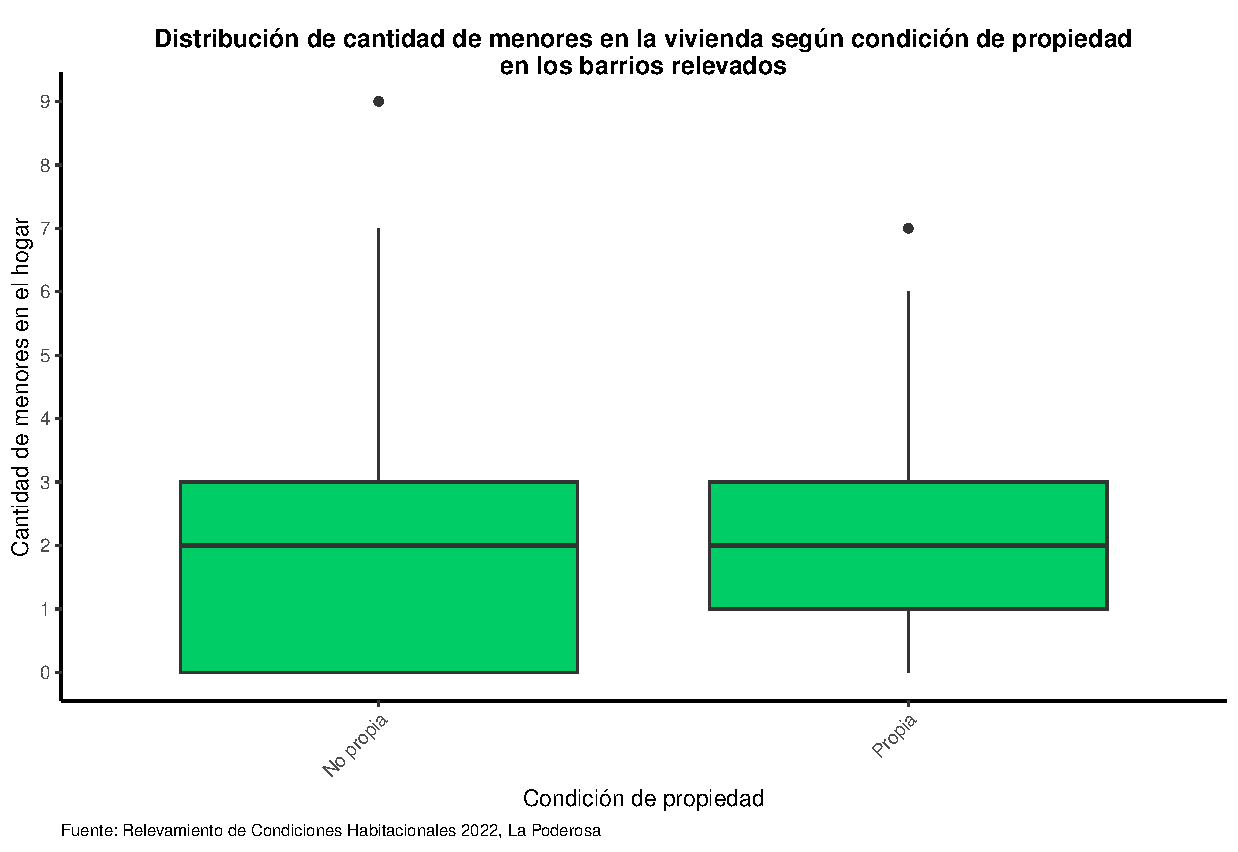
\includegraphics[height=.75\textheight]{graficas-pdf/boxplot-cant-menores-propiedad.pdf}}
                \only<3->{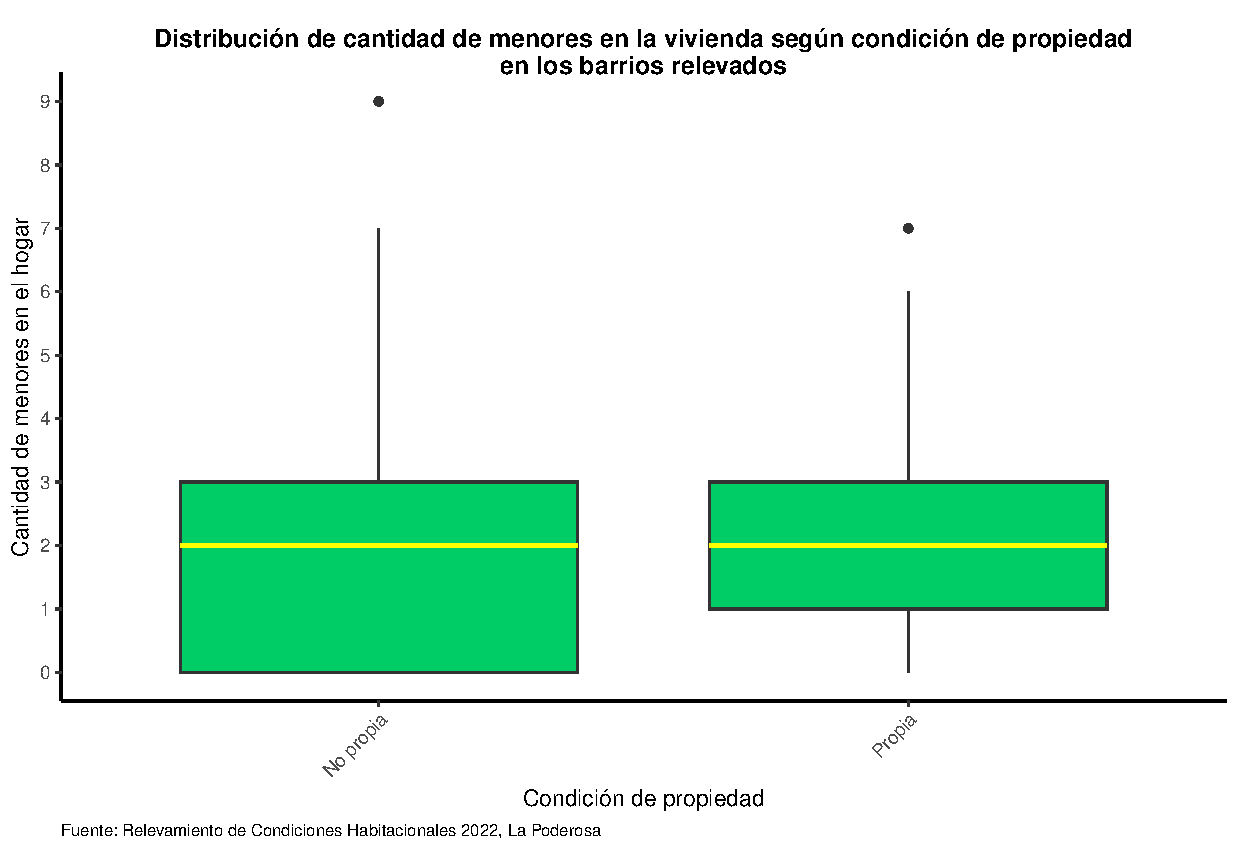
\includegraphics[height=.75\textheight]{graficas-pdf/boxplot-cant-menores-propiedad-med.pdf}}
            \end{overlayarea}
        \end{minipage}
        \begin{minipage}{.34\linewidth}
            \setlength{\leftmargini}{8pt}
            \small
            \begin{itemize}
                \item<2-> Distribución de la cantidad de menores \textbf{muy similar} entre ambas condiciones de tenencia.

                \item<3-> \textit{La mitad} de los hogares tiene \textbf{\textcolor{yellow!80!black}{hasta dos menores}} en ambos casos, y una \textit{cantidad promedio} de \textbf{1,8 menores} por vivienda.
                
                \item<4-> Alrededor de \textit{1 de cada 4} viviendas \textbf{no tiene} menores para ambas situaciones dominiales.
            \end{itemize}
        \end{minipage}
    \end{frame}

    \begin{frame}{Cantidad de menores en viviendas \textit{no propias}}
        \begin{minipage}{.65\linewidth}
            \begin{overlayarea}{\linewidth}{.75\textheight}
                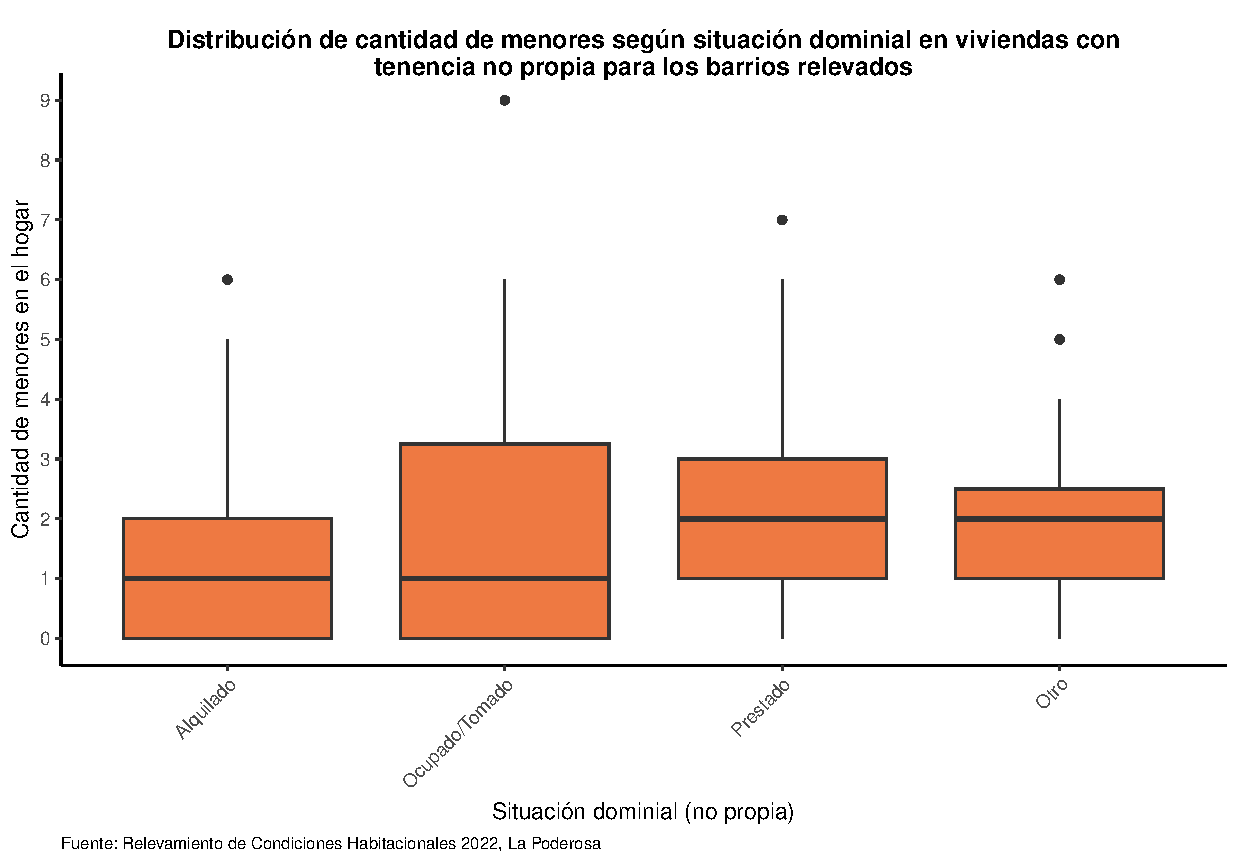
\includegraphics[height=.75\textheight]{graficas-pdf/boxplot-menores-nopropia-multivariado.pdf}
            \end{overlayarea}
        \end{minipage}
        \begin{minipage}{.34\linewidth}
            \setlength{\leftmargini}{8pt}
            \begin{itemize}
                \item<2-> Distribución de la cantidad de menores \textbf{similar} entre las distintas condiciones de tenencia no propias.

                \item<3-> \textbf{Levemente menor} cantidad de menores en promedio en \textit{viviendas alquiladas}, pero no significativa.
            \end{itemize}
        \end{minipage}
    \end{frame}

    \begin{frame}{Relación entre intentos de desalojo y la condición de tenencia}
        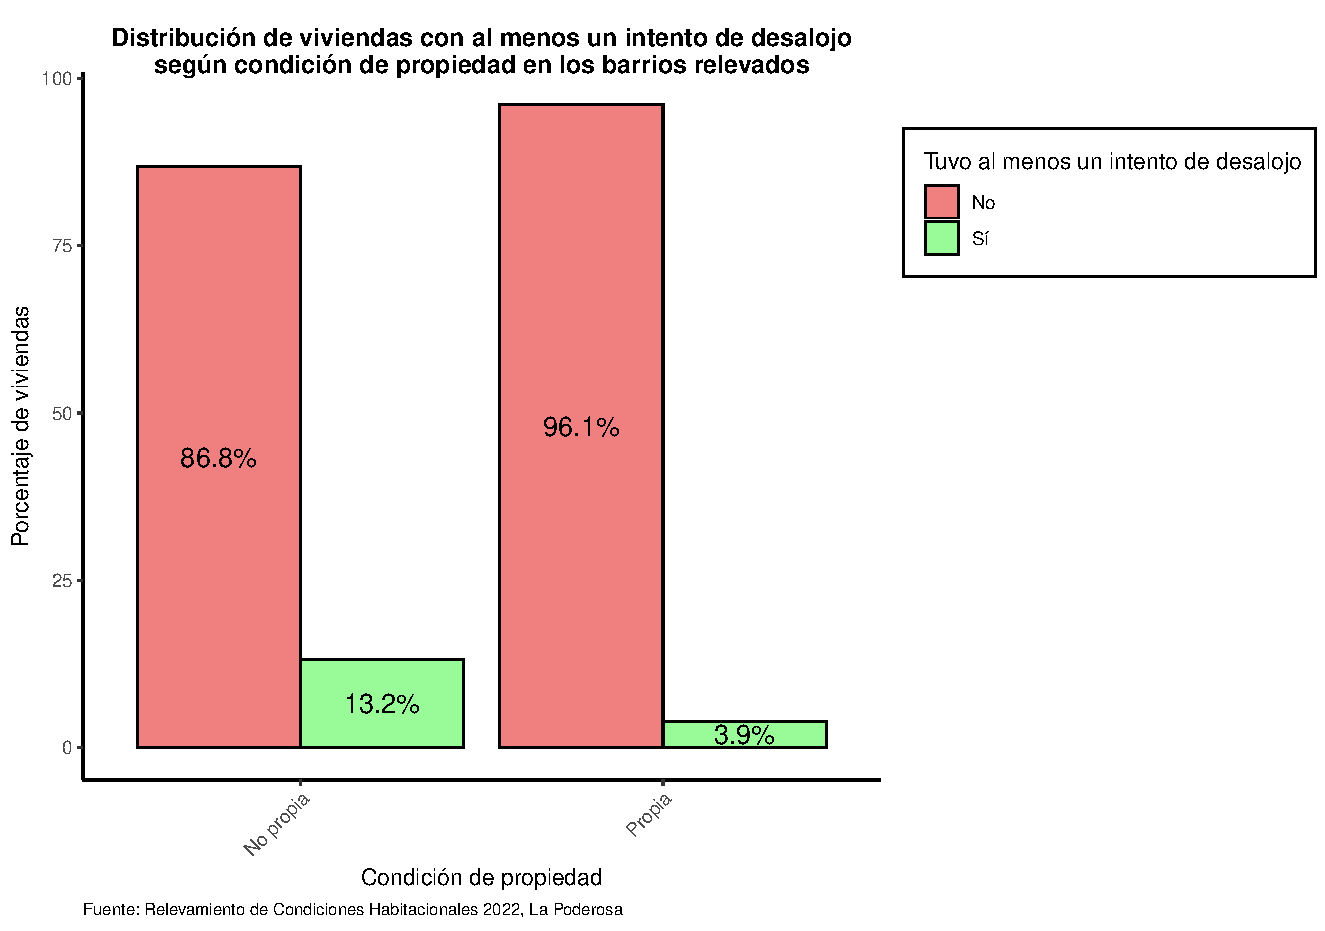
\includegraphics[height=.75\textheight]{graficas-pdf/desalojo-propiedad.pdf}\tikzmark{desalojo-propiedad}
        \begin{tikzpicture}[overlay, remember picture]
            \coordinate (a) at (pic cs:tipo-tenencia);
            \node[text width=8.5cm, align=left, anchor=north west] at ($ (a) + (-3.25,3.5) $) {\vbox{
                \begin{itemize}
                    \item<2-> En el grupo de viviendas no propias se registra un \textbf{10\% más} de familias que \textit{tuvieron al menos un intento de desalojo}, que en el grupo de viviendas propias.
                \end{itemize}
            }};
        \end{tikzpicture}

    \end{frame}

    \section{Conclusiones y próximos pasos}
    \begin{frame}
        \tableofcontents[currentsection]
    \end{frame} 

    \begin{frame}{Conclusiones}
        \setlength{\leftmargini}{8pt}
        \begin{itemize}
            \item<2-> La calidad de acceso a los servicios básicos como el agua y la luz es \textbf{muy precaria} en gran parte de las viviendas de los barrios relevados.
            \item<3->\textit{Un cuarto} de los jefes/as de hogar son \textbf{muy jóvenes} (hasta 19 años), posiblemente dificultando su formación y educación.
            \item<4-> Las características analizadas de las familias con \textit{tenencia propia} \textbf{no difieren demasiado} de las \textit{sin tenencia propia}, presentándose las mayores diferencias en tiempos de residencia algo mayores, y posibles intentos de desalojo.

            \item<5-> Los \textit{hogares inquilinos} presentan un \textbf{tiempo de residencia bajo} respecto al resto de familias en otras condiciones de tenencia. Además, la \textbf{dispersión de los valores del alquiler} en el territorio nacional podría ameritar un análisis más profundo.
        \end{itemize}
    \end{frame}

    \begin{frame}{Próximos pasos}
        \setlength{\leftmargini}{8pt}
        \begin{itemize}
            \item<2-> \textbf{Desarrollar políticas públicas} para \textit{mejorar la calidad de acceso a los servicios básicos} y para \textit{garantizar la educación} de los jefes/as de hogar jóvenes en los barrios populares.

            \item<3-> \textbf{Coordinar nuevos estudios} que recolecten información sobre \textit{desalojos} en los barrios populares con el fin de analizar la \textit{efectividad de políticas públicas} ya establecidas, como la creación del RENABAP.

            \item<4-> \textbf{Profundizar el análisis} en los \textit{hogares inquilinos} con datos actualizados y por regiones del país, a fin de determinar los \textit{factores que dificultan la permanencia prolongada} de estas familias en un mismo hogar.
        \end{itemize}
    \end{frame}

    \section*{}
    \begin{frame}
        \begin{center}
            \LARGE
            Muchas gracias \vspace{4pt}

            \small
            Advanced Analytics - Business Intelligence (Conosur), a cargo de Rubén Feffer\vspace{12pt}\pause

            \scriptsize
            \underline{Elaboración de gráficas}

            Antonella Grassi

            Emilia Moloeznik

            Ariel Fideleff
        \end{center}
    \end{frame}
\end{document}
